%TC:ignore
\documentclass{article}
\usepackage{graphicx} % Required for inserting images
\usepackage[colorlinks]{hyperref}
\usepackage{lscape}
\usepackage{setspace}
\usepackage[a4paper, total={16cm, 24cm}]{geometry}
\usepackage[style=numeric, sorting=none, maxbibnames=5]{biblatex}
\addbibresource{Thesis/references.bib}
\usepackage{pdflscape}
\usepackage[labelfont=bf]{caption}
\doublespacing
\title{\textbf{\line(1,0){350}
\\\huge{The Genetics of Mitochondrial Dysfunction in Sporadic Parkinson's Disease}
\\
\line(1,0){350}}}
\author{\textbf{Author:}
\\Thomas Brightwell
\\CID:01707452
\\
\\\textbf{Supervised by:}
\\Dr Toby Andrew & Dr Rahel Feleke
\\
\\
\\
\\
\\
\\
\\
\\MSc Human Molecular Genetics
\\Department of Metabolism, Digestion and Reproduction
\\Imperial College London
}
\date{August 22nd 2024}
\begin{document}
\begin{figure}
    
\includegraphics[width=0.5\linewidth]{Thesis/thesis images/IMPERIAL_logo_RGB_Blue_2024.png}
\end{figure}
\maketitle
\newpage
\paragraph{Declaration of originality}
This project report is submitted in partial fulfilment of the requirements for award of MSc in Human Molecular Genetics, Imperial College London. I hereby confirm that it is an original work, representing my own academic effort and that all sources have been fully acknowledged.
\paragraph{Declaration on use of Generative AI}
I hereby confirm that I have only used generative Artificial Intelligence (AI) according to the rules set out in the Academic Misconduct Policy and Procedure (point 14i). I confirm that all use of generative AI has been appropriately cited according to College guidelines and acknowledge that failing to do so or using generative AI in a manner different to that stipulated will constitute an examination offence and will be formally investigated.
\newpage
\begin{abstract}
Mitochondrial dysfunction has been shown to be central to Parkinson’s Disease (PD), both through causal familial PD (fPD) genes, and respiratory complex I inhibitors that cause the onset of PD symptoms (for example, animal models of PD). However, the mechanisms by which mitochondrial dysfunction may play a role in the aetiology of sporadic PD (sPD) are not well characterised, and depending upon the context, may be a cause or a consequence of the disease. Many studies have investigated the genetics of PD in general, but few directly investigate the relationship genetic variants have with mitochondrial function in sPD. This study uses a combination of genetic co-ocation and Differential Gene Expression (DGE) analysis to identify genes and pathways that are dysregulated in sPD patients. We employ fine scale genetic maps to precisely delineate disease loci coordinates centred upon lead SNPs from a large meta-analysis of Genome Wide Association Study (GWAS) to identify candidate functional target genes with expression Quantitative Trait Loci (eQTLs) that co-locate with the disease loci. We apply DGE to validate these cis-genes, and to test 43 clearly defined mitochondrial pathways for differential expression between sPD patients and controls. We show that there is large-scale downregulation of mitochondrial pathways in sPD patients (26 of 43 pathways tested), and we identify specific Nuclear Encoded Mitochondrial Genes (NEMGs) that are both differentially expressed in sPD patients and associated with the disease loci, which offer insight into the aetiology of sPD. We highlight \textit{NDUFAF3}, a respiratory complex I assembly factor, as a candidate target functional gene in sPD. 
\\
\\
\textbf{Abstract word count}: 256
\\
\textbf{Main text word count}: 11344
\end{abstract}
\newpage
\renewcommand{\abstractname}{Acknowledgements}
\begin{abstract}
I would like to thank my supervisors, Dr Toby Andrew and Dr Rahel Feleke for their fantastic supervision, support, and advice during my project (and Dr Toby Andrew specifically for his extensive feedback and guidance in writing this thesis), and for providing me with currently unpublished data for use in my analysis. I would also like to thank the collaborating lab at UCL, lead by Prof. Nikolas Maniatis, for their genetic maps. I would like to thank the other supervisors in the department who provided their input during our discussions \& monthly meetings, namely Dr Inês Cebola, Dr Hannah Maude, Dr Hatice Bahar Şahin, and Dr Shamith Samarajiwa. I would like to thank my friends and colleagues on the MSc Human Molecular Genetics course for enduring me as I used them as a sounding board and for some assistance with coding. Last, but not least, I would like to thank my long-suffering family for their unwavering support through my studies, something I would not be able to do without them.
\end{abstract}

\newpage
\tableofcontents
\listoftables
\listoffigures
\newpage
\section{Abbreviations}
BRAINEAC Brain Expression Almanac
\\DEGs Differentially Expressed Genes
\\DGE Differential Gene Expression
\\eQTL expression Quantitative Trait Locus
\\ETC Electron Transport Chain
\\fPD familial Parkinson's Disease
\\GEO Gene Expression Omnibus
\\GO Gene Ontology
\\GSEA Gene Set Enrichment Analysis
\\GTEx Genotype Tissue Expression Project
\\GWAS Genome Wide Association Study
\\GWASs Genome Wide Association Studies
\\IMM Inner Mitochondrial Membrane
\\iPSC induced Pluripotent Stem Cell
\\LD Linkage Disequilibrium
\\LDU Linkage Disequilibrium Units
\\MSA Multiple System Atrophy
\\NEMG Nuclear Encoded Mitochondrial Gene
\\OMM Outer Mitochondrial Membrane
\\PD Parkinson's Disease
\\PMI Post Mortem Index
\\PPMI Parkinson's Progression Markers Initiative
\\PRS Polygenic Risk Score
\\QTL Quantitative Trait Locus
\\QTLs Quantitative Trait Loci
\\RIN RNA Integrity Number
\\ROS Reactive Oxygen Species
\\scRNA single cell RNA
\\SN Substantia Nigra
\\SNP Single Nucleotide Polymorphism
\\sPD sporadic Parkinson's Disease
\\sQTL splicing Quantative Trait Locus
\\TAD Topologically Associated Domain
%TC:endignore
\newpage
\section{Introduction}
\subsection{Parkinson's Disease}
\subsubsection{Background}  
\label{subsubsec:Background}
Parkinson's Disease (PD), is a neurodegenerative disorder named after James Parkinson, who first formally described the disease in his 1817 ``An Essay on the Shaking Palsy"\cite{Parkinson2002AnPalsy}. The disease is primarily phenotypically characterised by tremors, bradykinesia, rigidity, and postural instability, although other non-motor symptoms are associated with the disease. These motor symptoms are caused by the fundamental pathophysiology of PD: the death of dopaminergic neurons in the Substantia Nigra (SN), a part of the basal ganglia. 
\\
\\PD is the second most common neurodegenerative disorder, behind Alzheimer's Disease. The 2021 Global Health Data exchange\cite{Ferrari2024Global2021} has yearly global incidence of PD to be 1.3 million cases. Global incidence is estimated at 0.15\%, but the age-related nature of PD can clearly be seen when this is split into the under and over 70 categories, with a prevalence of 0.06\% and 1.45\% respectively. This has profound implications for countries with ageing populations like the UK, where the incidence has increased by 41\% in the last 30 years \cite{Ferrari2024Global2021}. There is great impetus to understand the underlying molecular aetiology of PD, which could offer insights that lead to the development of new treatments.
\\
\\At the core of PD and many other conditions group together as synuceinopathies is the protein $\alpha$-synuclein and its aggregates. Lewy-Bodies are intracellular inclusions formed from $\alpha$-synuclein\cite{Spillantini1997-SynucleinBodies}, and are an important hallmark of PD. However, despite their widespread nature across PD subtypes and other diseases, the mechanism by which Lewy-Bodies cause pathological symptoms (if it does at all) is not fully clear\cite{Riederer2023LewyDisease}. It is however clear, that $\alpha$-synuclein itself is a crucial factor for PD.
\subsubsection{PD Sub-types and Terminology}
\label{subsubsec:PDtypes}
PD is often distinguished clinically by the age of onset, but there is not a consensus on the definition of early or late onset\cite{Riboldi2022AParkinsonism}. Usually, those under 50 years are considered to have early-onset Parkinson's, with those who develop later symptoms considered to have late-onset PD, but some use a threshold of 40 years instead\cite{Ferguson2016Early-onsetStudy}.
\\
\\Parkinson's Disease is divided into three genetic classifications: Familial Parkinson's Disease (fPD), divided into early-onset and classical, Sporadic Parkinson's Disease (sPD), and GBA1-type PD\cite{Tolosa2021ChallengesDisease}. fPD is a monogenic disorder, with certain key genes being responsible for nearly all cases of fDP, outlined in \hyperref[tab:fPDgenes]{Table 1}. Depending on the gene responsible for the specific patient's fPD, it can inherited in either a autosomal dominant or autosomal recessive fashion\cite{Day2021ThePractice}. GBA1-type PD is distinct from standard fPD because it does not follow a standard monogenic inheritance pattern and has very variable penetrance. sPD (sometimes also called idiopathic PD) is a complex trait, with considerable environmental influence and a heritable component\cite{Nalls2019IdentificationStudies}. Many different environmental factors have been found to influence sPD risk\cite{Costa2023ParkinsonsDisorder}, from pesticide exposure to caffeine intake, however age is the most important. sPD accounts for the majority of PD cases - up to 90\% of PD patients do not have a family history of the disease\cite{Inamdar2007ParkinsonsBeyond}. This means that most cases of PD do not have a clear aetiology. 
\\
\\There is significant overlap between patients who have a ``Parkinsonism", for example those who develop Lewy-Body dementia first, and subsequently PD-like symptoms\cite{Jellinger2018DementiaControversies}, and those who have PD first and develop other symptoms later. There are many different Parkinsonism's - a subset of synucleiopathies that include diseases such as Multiple System Atrophy (MSA)\cite{Hayes2019ParkinsonsParkinsonism}. These diseases have a shared aetiology of $\alpha$-synuclein protein misfolding. Whilst fPD can be mitigated in the population by genetic counselling and careful planning, sPD is intrinsically harder to predict and counsel. This study specifically investigated the genetic component of sPD, in an effort to identify the target genes of sPD risk loci described in Nalls et al.\cite{Nalls2019IdentificationStudies}. Understanding the molecular nature of common disease has the potential to highlight important variants and genes that can be targeted for further functional validation, and if promising, therapeutic treatment.
\subsubsection{The Genetics of Parkinson’s Disease}
PD is a disease with great genetic heterogeneity, along with the previously discussed clinical heterogeneity discussed above. 
\paragraph{Genetics of fPD}Up to 17 genes have been discovered as causes of fPD\cite{Day2021ThePractice}, with most following an autosomal dominant pattern of inheritance, and a minority following a autosomal recessive pattern. The first discovered fPD gene was \textit{SNCA}, which codes for $\alpha$-synuclein, thanks to the rare and highly penetrant nature of variants in \textit{SNCA}. In contrast, the most common fPD mutations are in \textit{LRRK2}\cite{Klein2012GeneticsDisease}. Each of the genes identified as causing fPD offers insight into the mechanisms underlying PD, and many of these genes are associated with mitochondrial function (discussed in Section \hyperref[subsec:mitochondria]{2.3}). The most common causes of fPD are shown below in Table 1:
%TC:ignore
\begin{table}[h]
    \label{tab:fPDgenes}
    \centering
    \caption{Brief summary of the five most important familial Parkinson's Disease genes, including their corresponding protein, their cellular role, and if they are NEMGs.}
    \begin{tabular}{|p{2.5cm}|p{4cm}|p{6cm}|p{1.5cm}|}
        \hline
        Gene Symbol & Protein name & Role(s) & NEMG \\ \hline
        \textit{SNCA} & $\alpha-$Synuclein & Synaptic vesicle trafficking, SNARE complex interactions & No \\ \hline
        \textit{LRRK2} & Leucine Rich Repeat Kinase 2 & Serine-Threonine kinase, involved in many processes in the neuron & No \\ \hline
        \textit{PINK1} & PTEN Induced Kinase 1 & Serine-Threonine kinase, major role in mitochodrial dynamics & Yes\\ \hline
        \textit{PRKN} & Parkin & Ubiquitin ligase, major role in mitochondrial dynmaics & Yes\\ \hline
        \textit{PARK7} & Parkinsonism Associated Deglycase & Senses and protects against oxidative stress & Yes\\ \hline
    \end{tabular}
\end{table}
%TC:endignore
\\Three of the five most common fPD genes are Nuclear Encoded Mitochondrial Genes (NEMGs), based on the MitoCarta3.0\cite{Rath2021MitoCarta3.0:Annotations} list of NEMGs. The two remaining genes, \textit{SNCA} and \textit{LRRK2}, both have many interactions with the mitochondria, which will be discussed further in this section. This underscores the importance of mitochondria in fPD.
\paragraph{Genetics of sPD}The genetics of sPD are less well characterised compared to fPD. Many individual studies have investigated the heritable component of sPD, the largest of which is a 2019 meta-analysis of PD-GWASs by Nalls et al. \cite{Nalls2019IdentificationStudies}. In their study, they identified 90 lead Single Nucleotide Polymorphisms (SNPs) most significantly associated with PD. This meta analysis combined 16 case-control studies of PD, with a total of 37.7 thousand cases, and 1.4 million controls. They employed a conditional and joint analysis strategy - i.e.  to conduct an additional conditional analysis on the identified loci to find potential secondary SNPs, then jointly test their combined effect on the phenotype\cite{Yang2012ConditionalTraits}. This method improves the explained proportion of heritability by capturing more variants with smaller effects. The authors estimated a Polygenic Risk Score (PRS) that explained a median 26\% of the heritability in liability for PD, with estimates ranging from 16-36\%. However, the authors do note that this is highly dependent on the prevalence of PD in the population, and on the inclusion of exclusion of rare variants within the calculation.
\subsection{Inflammation in PD}
\label{subsec:inflammation}
Inflammation is thought to play a major role in PD, but the exact relationship between neuroinflammation and PD is not fully understood, as discussed by Marogianni et al.\cite{Marogianni2020NeurodegenerationDisease}. Chronic inflammation is observed in PD brains, as cell death leaves debris in the surrounding tissue, attracting microglia to clear the debris\cite{Pajares2020InflammationImplications}. However, microglia can also promote cell death via apoptosis, and are known to be key to synaptic pruning. There is evidence for a feedback loop between these events, where cell death creates debris, attracting microglia and causing inflammation, leading to greater cell death, and the cycle repeats.
\\
\\The gut-brain axis is a major point of interest for understanding the initial triggers of PD, and inflammation in the bowel is potentially a contributing factor to the development of PD\cite{Marogianni2020NeurodegenerationDisease}.
Additionally, $\alpha$-synuclein aggregates are thought to trigger an inflammatory response. It has been proposed that this explains the non-motor symptoms that can occur decades earlier in patients\cite{Forloni2023AlphaInflammation}. However, the cause and effect is not clearly established, and inflammation may be more of a symptom than a cause of PD\cite{Pajares2020InflammationImplications}, but there is evidence that microglial-mediated inflammation is important for the progression of PD\cite{Isik2023MicrogliaDisease}.
\subsection{The role of mitochondria in PD}
\label{subsec:mitochondria}
\subsubsection{The Origin \& Function of Mitochondria and Nuclear Encoded Mitochondrial Genes}
The mitochondria is a double-membrane bound organelle, common to almost all eukaryotes (aside from a few unicellular parasites that are theorised to have lost them\cite{Karnkowska2016AOrganelle}). It is now widely accepted that the origin of the mitochondria was an endosymbiotic event\cite{Martin2015EndosymbioticOrigin.}.The ancestor to all eukaryotic cells internalised a bacterial cell which began to work in concert with its host to the benefit of both cells. As it has an extracellular origin, the mitochondria has a key feature that other non-nuclear organelles lack: its own genome. The mitochondrial genome is very small, with only 37 genes encoded within\cite{Taanman1999TheReplication}. However, there are many more genes not encoded by the mitochondrial genome that still localise to the mitochondria and perform their cellular role there.
\\
\\The latest 3.0 version of MitoCarta \cite{Rath2021MitoCarta3.0:Annotations} lists 1136 human protein-coding genes that have strong evidence for localisation to the mitochondria. This highlights how the overwhelming majority of mitochondrial genes have migrated to the nucleus over the course of mitochondrial evolution. Another dataset from the Mitochondrial Biology Unit at MRC Cambridge called the Integrated Mitochondrial Protein Index (IMPI), available both from their website \href{https://www.mrc-mbu.cam.ac.uk/research-resources-and-facilities/impi}{here} and through their MitoMiner tool\cite{Smith2016MitoMinerDatabase}, also classifies genes that are associated or ancillary to the mitochondria, for a total of 1,966. This database also includes the two genes from \hyperref[tab:fPDgenes]{Table 1} that are not listed as NEMGs in MitoCarta3.0 - \textit{SNCA} \& \textit{LRRK2} - which emphasises the importance of the definition used.
\\
\\Mitochondria are involved in many cellular processes, but some of the key pathways for disease are ATP production by oxidative phosphorylation, apoptosis, and cell signalling\cite{Rossmann2021MitochondrialDisease}. Additionally, the production of Reactive Oxygen Species (ROS) as a byproduct of oxidative phosphorylation is an important factor for both aging and disease\cite{Brieger2012ReactiveDisease}. Diseases linked with mitochondria can therefore have a wide range of phenotypes - from metabolic disorders\cite{Bhatti2017MitochondrialStrategies} to autoimmune diseases\cite{Xu2020EmergingDiseases}, and most importantly for this study, neurodegenerative disorders\cite{MonzioCompagnoni2020TheDisease}.
\subsubsection{$\alpha$-Synuclein pathology}
\label{subsubsec:synuclein}
As described in \hyperref[subsubsec:Background]{2.1.1}, $\alpha$-synuclein is fundamental to PD and other synucleinopathies, but its role in both healthy function and disease state in the brain is not fully understood. $\alpha$-Synuclein can take multiple forms, from single monomers, to oligomers, to full amyloid fibrils\cite{Mehra2019-SynucleinPathogenesis}. Soluble monomers of $\alpha$-synuclein binds to lipid membranes, which includes both vesicles and the mitochondrial membrane\cite{Burre2018Cell-Synuclein}. It has been shown that the seeding events that convert functional $\alpha$-synuclein into the oligomeric form that acts as a toxin\cite{Choi2022PathologicalToxicity} occurs at the mitochondrial membrane. Another way that $\alpha$-synuclein is thought to act is through inflammation, as $\alpha$-synuclein can trigger the NLRP3 inflammasome complex\cite{Forloni2023AlphaInflammation}. $\alpha$-Synuclein has been proposed to play a role in many different PD-linked pathways, some of which are mitochondrial, discussed in section \hyperref[subsubsec:mitochondria]{2.3.3}.
\subsubsection{Mitochondrial dysfunction}
\label{subsubsec:mitochondria}
The first evidence for mitochondrial involvement in PD emerged in 1983, when a complex I inhibitor produced as a byproduct of heroin production was shown to cause PD-like symptoms\cite{Langston1983ChronicSynthesis}. Mitochondria are now considered one of the most important factors in both fPD and sPD\cite{Henrich2023MitochondrialPotential}, and many of the genes responsible for fPD are mitochondrial. Whilst there are many (and not mutually exclusive) different theories for the specifics of how mitochondria are involved in the aetiology of PD, some of the of the most convincing are outlined here: Mitophagy, Mitochondrial Dynamics, and Oxidative Stress.
\paragraph{Mitophagy}Two genes, \textit{PINK1} and \textit{PRKN} (which codes for the Parkin protein), are common causes of fPD when mutated\cite{Malpartida2021MitochondrialTherapy}. PINK1 is a kinase localised to the mitochondrial membrane\cite{Narendra2010PINK1Parkin}, and Parkin is a cytosolic ubiquitin ligase\cite{Narendra2008ParkinAutophagy}. Both genes interact together to recognise and flag impaired mitochondria for degradation. Under normal conditions, PINK1 is cleaved by factors in the mitochondrial matrix and Inner Mitochondrial Membrane (IMM), allowing it to degraded by the proteosome\cite{Pickles2018MitophagyMaintenance}. However, under stress conditions, PINK1 becomes stabilised on the Outer Mitochondrial Membrane (OMM) and can perform its function of phosphorylating Parkin. Once phosphorylated, Parkin can then be recruited to the OMM, where it acts as a signal for mitophagy. As mutations in either of these genes can cause fPD it implies that mitochondrial degradation and mitophagy play an important role in PD. Additionally, other PD genes like \textit{GBA1}, \textit{SNCA}, and \textit{LRRK2} interact with this pathway to impair mitophagy when mutated\cite{Malpartida2021MitochondrialTherapy}. The mechanistic details are less clear, but impaired mitochondrial homeostasis may lead to an increase of stress factors on the cell, leading to apoptosis\cite{Eldeeb2022MitochondrialDisease}.
\paragraph{Mitochondrial Dynamics}Mitochondrial dynamics are important for maintaining the delicate balance of a neuronal cell\cite{Chen2009MitochondrialDiseases}. Due to the unique morphology and energetic requirements of neurons, a cell keeping the right number of mitochondria in the right locations is a complex and tightly regulated process. The two previously mentioned genes \textit{PINK1} and \textit{PRKN} have a role in determining mitochondrial fission in addition to the earlier described role in mitophagy, and mitochondrial dynamics and mitophagy are inherently linked\cite{Archer2013MitochondrialDiseases}. Disrupted fission processes increases oxidative stress on the cell and can lead to apoptosis. \textit{LRRK2}, another fPD gene promotes mitochondrial fission by phosphorylation of Drp1. The most common single cause of fPD is a specific G2019S mutation in \textit{LRRK2} that causes over-activity and therefore aberrant mitochondrial fission\cite{Su2013InhibitionMutation}. $\alpha$-Synuclein is also thought to play a role in many mitochondrial dynamics processes, including inhibition of fusion and mitochondrial transport\cite{Valdinocci2019IntracellularDisease}. Overall, there is clear evidence that mitochondrial dynamics are central to PD, although the mechanisms for this action are not yet fully understood.
\paragraph{Oxidative Stress}
\label{para:oxidative}
ROS are associated with many poor outcomes for cells. Excess ROS can cause major damage to both organelles and macro-molecules, which contributes to many different diseases, including neurodegenerative diseases\cite{Brieger2012ReactiveDisease}. Normally, cells that accumulate a critical threshold of damage undergo apoptosis, and this may be the cause for the characteristic death of dopaminergic neurons in the SN\cite{Subramaniam2013MitochondrialDisease}. Many of the toxins that can trigger onset of PD or PD-like symptoms are inhibitors of some factor in the Electron Transport Chain (ETC), most commonly complex 1\cite{Subramaniam2013MitochondrialDisease}.
\\
\\Complexes I \& III are the two main locations of ROS production in the mitochondria\cite{Murphy2009HowSpecies}, and therefore the cell. Complex I is is a common thread between many different genes that cause fPD. \textit{SNCA}, \textit{PINK1}, \textit{PARK2},\textit{7}\&\textit{8} are all fPD genes shown to cause complex I impairment\cite{Subramaniam2013MitochondrialDisease}. The complex I inhibitor Rotenone has been used to create PD models in rodents since the 2000s\cite{Betarbet2000ChronicDisease}, and there is evidence that specific disruption of complex I in dopaminergic neurons reproduces PD symptoms\cite{Gonzalez-Rodriguez2021DisruptionParkinsonism}. It is thought that disruption of complex I leads to an increased production of ROS, which increases the stress on the cell, leading to apoptosis\cite{Subramaniam2013MitochondrialDisease}.
\\
\\The toxic oligomeric form of $\alpha$-synuclein also leads to the generation of ROS, which can then go on to damage other critical cell compartments \cite{Choi2022PathologicalToxicity}. There is evidence for a feedback loop between $\alpha$-synuclein, ROS, iron and neuromelanin, which propagates the spread of neurodegeneration in a PD brain\cite{JansenvanRensburg2021ToxicTurmeric}. The increase in ROS also damages the mitochondrial genome, which may lead to a build-up of deleterious mutations. It has been shown that PD patients have higher frequencies of mtDNA deletions in the SN than other regions of the brain\cite{Bender2006HighDisease}. Together, these make a strong case for dysfunction in the ETC being implicated in the aetiology of PD.
\subsection{Genetic Analysis Techniques}
\subsubsection{Linkage Disequilibrium and Association Mapping}
\label{subsubsec:linkage}
Linkage is the phenomenon of genetic loci that are physically close to each other on the same chromosome tending to be inherited together, disobeying the law of independent assortment. This occurs because recombination has a lower chance of occurring between two loci that are next to each other, so linked alleles are typically inherited together on a single haplotype. Linkage Disequilibrium (LD) is a related, but distinct, phenomenon of two or more genetic loci showing non-random association with each other\cite{Slatkin2008LinkageFuture} in a population. Linkage is a phenomenon of family data, but LD is observed in both family and population data, reflecting historical patterns of recombination. Accordingly, a linkage map shows recombination events with a family (extant recombination events)\cite{Lynn2004VARIATIONRECOMBINATION}, and a LD map shows a the pattern of recombination across a population - historical recombination events. This is population-specific - after a population has diverged, the pattern of recombination in each will be diverge.
\\
\\Consideration of LD is central to this study is because a GWAS does not test every single possible variant in the genome - as this would be impractical for both sequencing and frequentist significance. A GWAS instead relies on a combination of imputation\cite{Dehghan2018Genome-WideStudies} for genotypes absent on the array and genotyped marker variants that are in high LD with the true functional variant(s) (as it is very unlikely that the functional variant itself is tested). This is an indirect test of association\cite{Weiss2000HowSNPs}. Accordingly, the lower the LD between a functional variant and the marker variant, the less power the study has, to the limit of no power if there is no LD. Genomic studies often assume the common variant common disease hypothesis. This can limit results, as it is unlikely that all common diseases have corresponding functional common variants\cite{Bodmer2008CommonDiseases}. Some GWASs, like the Nalls et al. study\cite{Nalls2019IdentificationStudies}, attempt to address this problem by also conducting rare variant mining and burden tests. This study addresses some of these issues by employing population specific high-resolution genetic maps\cite{Maniatis2004PositionalDisequilibrium.} to find the complete region of LD around the 90 PD lead SNPs. This is one method among many that potentially allows the testing of all variants with the region of LD, instead of just the lead SNP, improving the ability to detect genes functionally associated with the disease loci.
\subsubsection{Quantitative Trait Loci}
\label{subsubsec:QTL}
A Quantitative Trait Locus (QTL)is a region or variant in the genome that is associated with a mean difference in a quantitative trait between individuals. For a given set of samples, a QTL can be implemented by linear regression of the trait being investigated against the genotype of a particular loci\cite{Duffy2017AnalysisLoci}. Classically, QTLs were considered for phenotypic traits such as height, but QTL analysis can also be employed for molecular traits such as gene expression. The study hypothesis is that the molecular QTL may act as an intermediary risk factor for complex traits. This method has been particularly useful when attempting to understand GWAS results that highlight certain regions of the genome and corresponding implicated genes as associated with a complex trait. QTL analysis provides a potential explanation for how the discovered loci interact with the complex traits\cite{Neumeyer2020StrengtheningLoci}. In this study, the complex trait being considered is sPD, and the quantitative trait used as an intermediary is the mRNA expression level of neighbouring genes, so the QTLs are specifically expression Quantitative Trait Loci (eQTLs). For more details on the eQTL analysis see \hyperref[subsec:eQTL]{methods section 3.2}. eQTLs are used in this study to implicate causal genes for the lead SNPs found in the Nalls et al.\cite{Nalls2019IdentificationStudies} meta-analysis, which is achieved by co-locating the QTL with the disease loci.
\subsubsection{Co-location}
\label{subsubsec:co-location}
The aim of a co-location analysis is to find a an eQTL variant that is in the same genetic position as a disease associated location or variant\cite{Cano-Gamez2020FromDiseases}. As these variants share the same genetic position, they are co-located. There are multiple methods for co-localisation - with some based entirely on genome-wide summary statistics. In this study we are using a European genetic map\cite{Maniatis2004PositionalDisequilibrium.} to define PD loci coordinates, centred upon the lead SNPs from Nalls et al.\cite{Nalls2019IdentificationStudies} to test for association with a change in gene expression. By first defining the genetic and physical coordinates of these loci, we can then search for eQTL \textit{cis}-gene associations within the same locus. To illustrate this idea, Figure 1 shown an example locus around one of the lead SNPs from Nalls et al.\cite{Nalls2019IdentificationStudies}
%TC:ignore
\begin{figure}[!h]
    \centering
    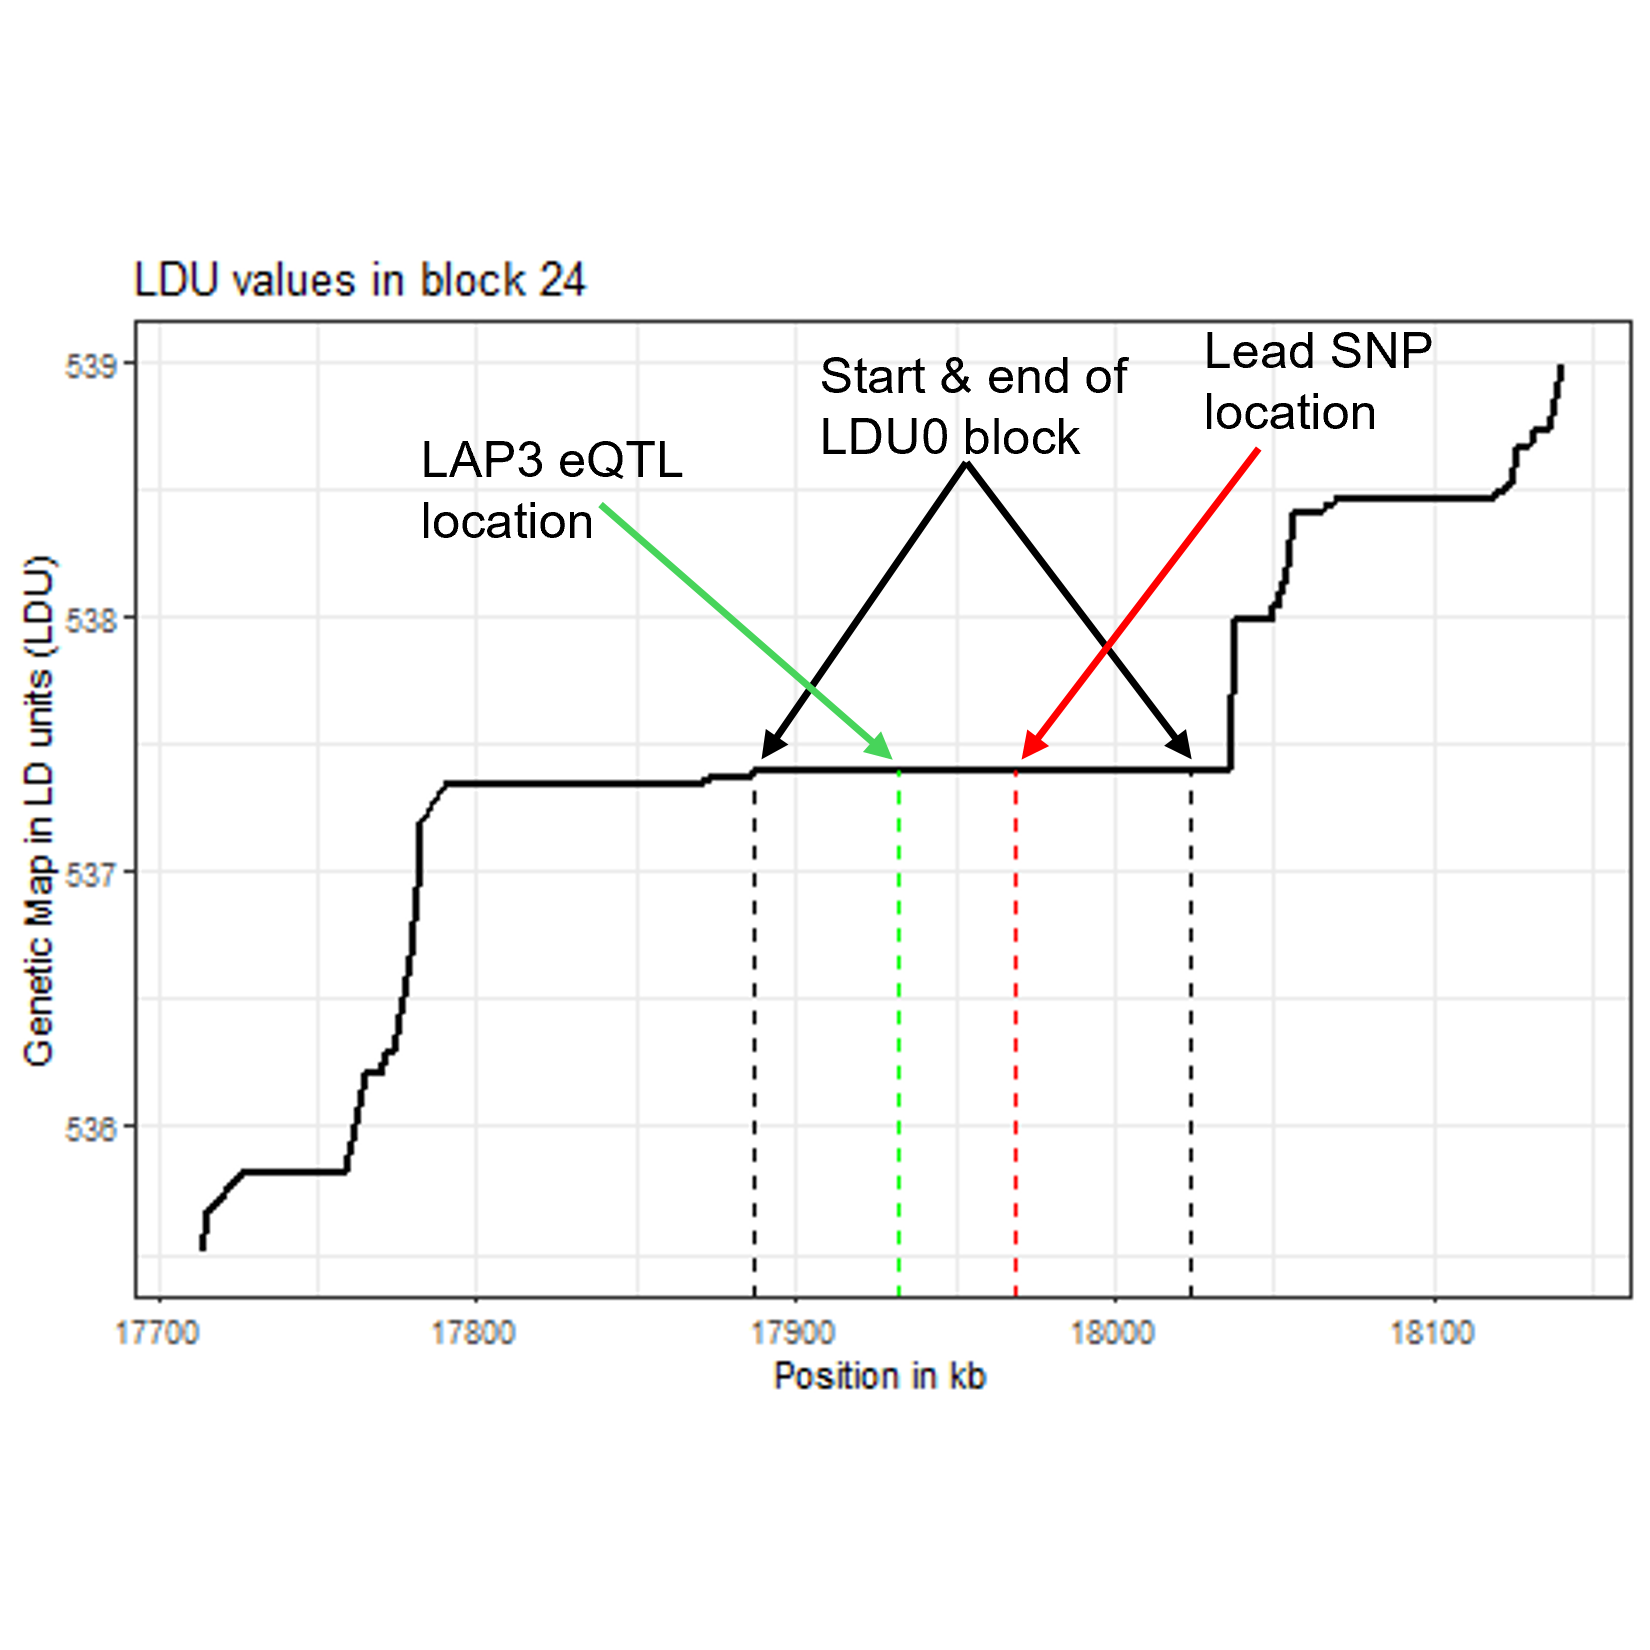
\includegraphics[width=1\linewidth]{Thesis/thesis images/exampleblock.png}
    \caption{Linkage disequilibrium step and block graph (in cumulative LD units) against physical distance (in kilobases, from hg37) for LD block 24 on chromosome 4p15. The Nalls et al. lead SNP and eQTL for cis-gene LAP3 colocate, since they share the same genetic location and LD block. The dotted lines show 3 things:The eQTL location is shown in green, the lead SNP is shown in red, and the boundaries of the region with no LD breakdown are shown in black.}
    \label{fig:block}
\end{figure}
%TC:endignore
\\
\\In \hyperref[fig:block]{Figure 1}, the vertical steps in the line show places where historical recombination has occurred, whilst the plateaus show regions where there has been no historical recombination. As the physical lead SNP and LAP3 eQTL location are both on the same block, there has not been any recombination between these two points. This means that both are at the same genetic location. Therefore, the disease associated variant and the eQTL have shown strong evidence of co-location.
This process is facilitated by high-resolution genetic maps\cite{Maniatis2004PositionalDisequilibrium.}, and follows a similar method to that described by Maude et al.\cite{Maude2021NewDiabetes.}
\newpage
\subsubsection{Pathway \& Network Analyses}
\label{subsubsec:pathwaysandnetworks}
The biological interpretation of multiple individual genes identified in a study can be very difficult, especially when conducting a genome-wide study with potentially hundreds of significant target genes. Two main approaches to reducing the complexity of results are network and pathway analysis. Network analyses cluster genes based on their interactions, creating networks of genes encoding proteins that all have various interactions with each other\cite{Maayan2011IntroductionBiology}, such as protein-protein interacts or co-expression. Pathway analyses instead cluster genes based on shared functions and roles in the cell\cite{Garcia-Campos2015PathwayArt} - for example, grouping all genes that code for a part of the TCA cycle into specific TCA cycle group. The defined interaction in network analyses are often predicted, whereas the pathways in pathway analyses are usually manually curated. The difference in approach between network and pathway analyses lend themselves to different questions. As pathway analyses are conducted on pre-defined pathways, these can be used for hypothesis driven research, whereas network analyses are more useful for discovery driven research, as the end point is not pre-defined.
\\
\\There are many different database that can be used for classifying genes in a pathway analysis, such as Gene Ontology (GO)\cite{Ashburner2000GeneBiology}, or the Kyto Encyclopedia of Genes and Genomes (KEGG)\cite{Kanehisa2016KEGGAnnotation}. Many tools exist for the analysis of any given set of genes in comparison to the chosen database, but in this study we will be using Gene Set Enrichment Analyis (GSEA)\cite{Subramanian2005GeneProfiles}. The ranking approach of GSEA allows for detection of small differences across multiple genes within the same pathway, as the score for a pathway can be affected by both outliers with extreme expression differences, and small differences within many genes. It is worth noting that the power to detect significant results in GSEA is heavily contingent on well defined and functionally meaningful pathways, and poorly-choses datasets will likely not yield any meaningful results. See section \hyperref[subsec:pathways]{3.4} for more details on the GSEA performed in this study. Additionally, a network analysis was conducted using STRING\cite{Neumeyer2020StrengtheningLoci}.
\subsection{Hypothesis \& Study Aims}
\subsubsection{Hypothesis}
\label{subsubsec:hypothesis}
The study hypothesis being investigated is:
\\
\\
Mitochondrial dysfunction plays a major role in the onset and pathophysiology of sporadic Parkinson’s Disease via multiple identifiable molecular pathways.
\\
\\Mitochondrial (dys)function is likely to play a key role in the aetiology of neurological diseases\cite{Bartman2024MitochondrialDiseases}, and particularly neurodegenerative diseases such as Alzheimer's disease and PD\cite{MonzioCompagnoni2020TheDisease}. However, it is less certain whether mitochondrial dysfunction plays a causal role, or is a consequence of the disease, or both. As discussed in section \hyperref[subsubsec:mitochondria]{2.3}, there is strong evidence to suggest that multiple different potential causal pathways that could modulate PD in patients. However, what is less clear is the role genetics may have in shaping mitochondrial dysfunction in sPD, and accordingly, this is what this study is designed to test. The hypothesis of mitochondrial dysfunction affecting sPD is visually summarised in Figure 2.
\begin{figure}[h]
    \centering
    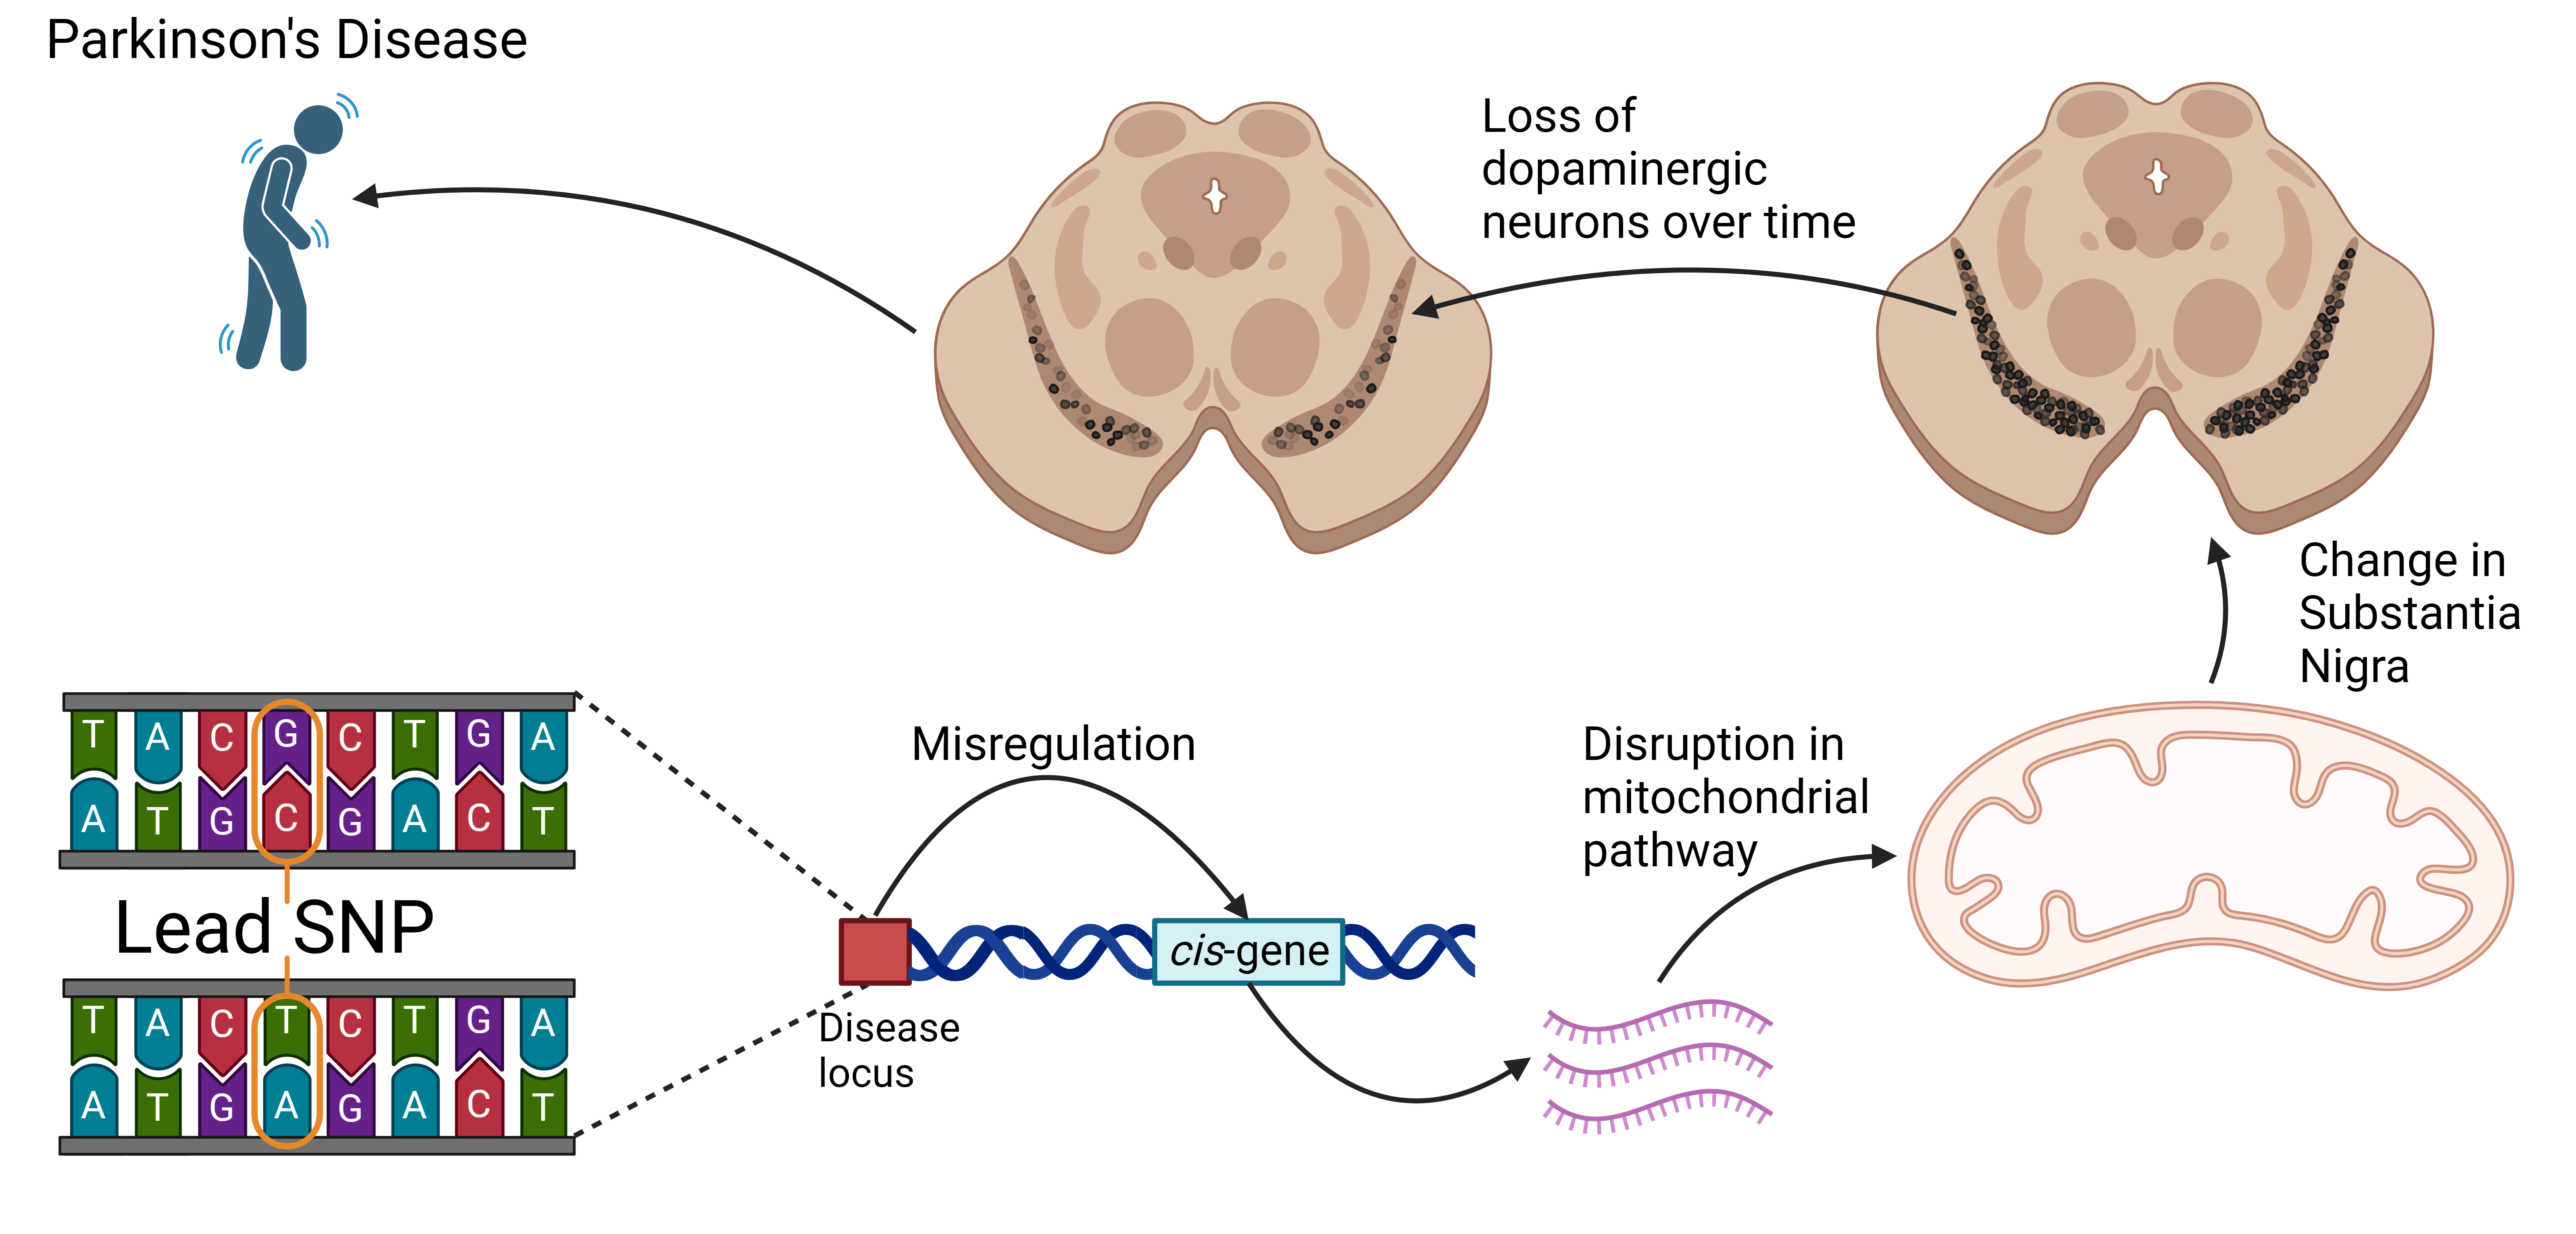
\includegraphics[width=1\linewidth]{Thesis/thesis images/Visualhypothesis.png}
    \caption{Summary of the hypothesis being tested in this study. The GWAS lead SNPs are located at disease loci, which cause misregulation of \textit{cis}-genes. This change in expression level disrupts mitochondrial pathway(s), affecting the SN and promoting dopaminergic neuron cell death. This in turn leads to the onset of PD symptoms.}
    \label{fig:enter-label}
\end{figure}
\subsubsection{Research Aims}
\label{subsubsec:Aims}
There are four related research aims in this study:
\begin{enumerate}
    \item Using the lead SNPs identified by Nalls et al.\cite{Nalls2019IdentificationStudies}, identify the precise genetic and physical location boundaries for all the disease loci. These loci will contain the putative functional variant(s) that causally contribute to sPD risk detected in the GWAS. Additionally, conduct a coding variants search for the loci containing exons.
    \item Conduct disease-eQTL co-location analyses to identify \textit{cis}-genes that are both associated and co-located with the disease loci defined in aim 1 using population based datasets (GTEx and BRAINEAC).
    \item Validate disease-eQTL\textit{cis}genes using observational (GEO) and experimental (PPMI) expression data to conduct Differential Gene Expression (DGE) analysis for the co-located eQTL-\textit{cis}genes identified in aim 2.
    \item Conduct pathway analysis and GSEA\cite{Subramanian2005GeneProfiles} to test for enrichment of mitochondrial pathways in sPD patients, and specifically the enrichment of Nuclear Encoded Mitochondrial Genes (NEMGs) for disease-affected \textit{cis}-genes in aim 3.
\end{enumerate}
Figure 3 provides an overview for the workflow of this project, summarising the methods undertaken to address the four aims.
\newpage
%TC:ignore
\begin{figure}[!h]
    \centering
    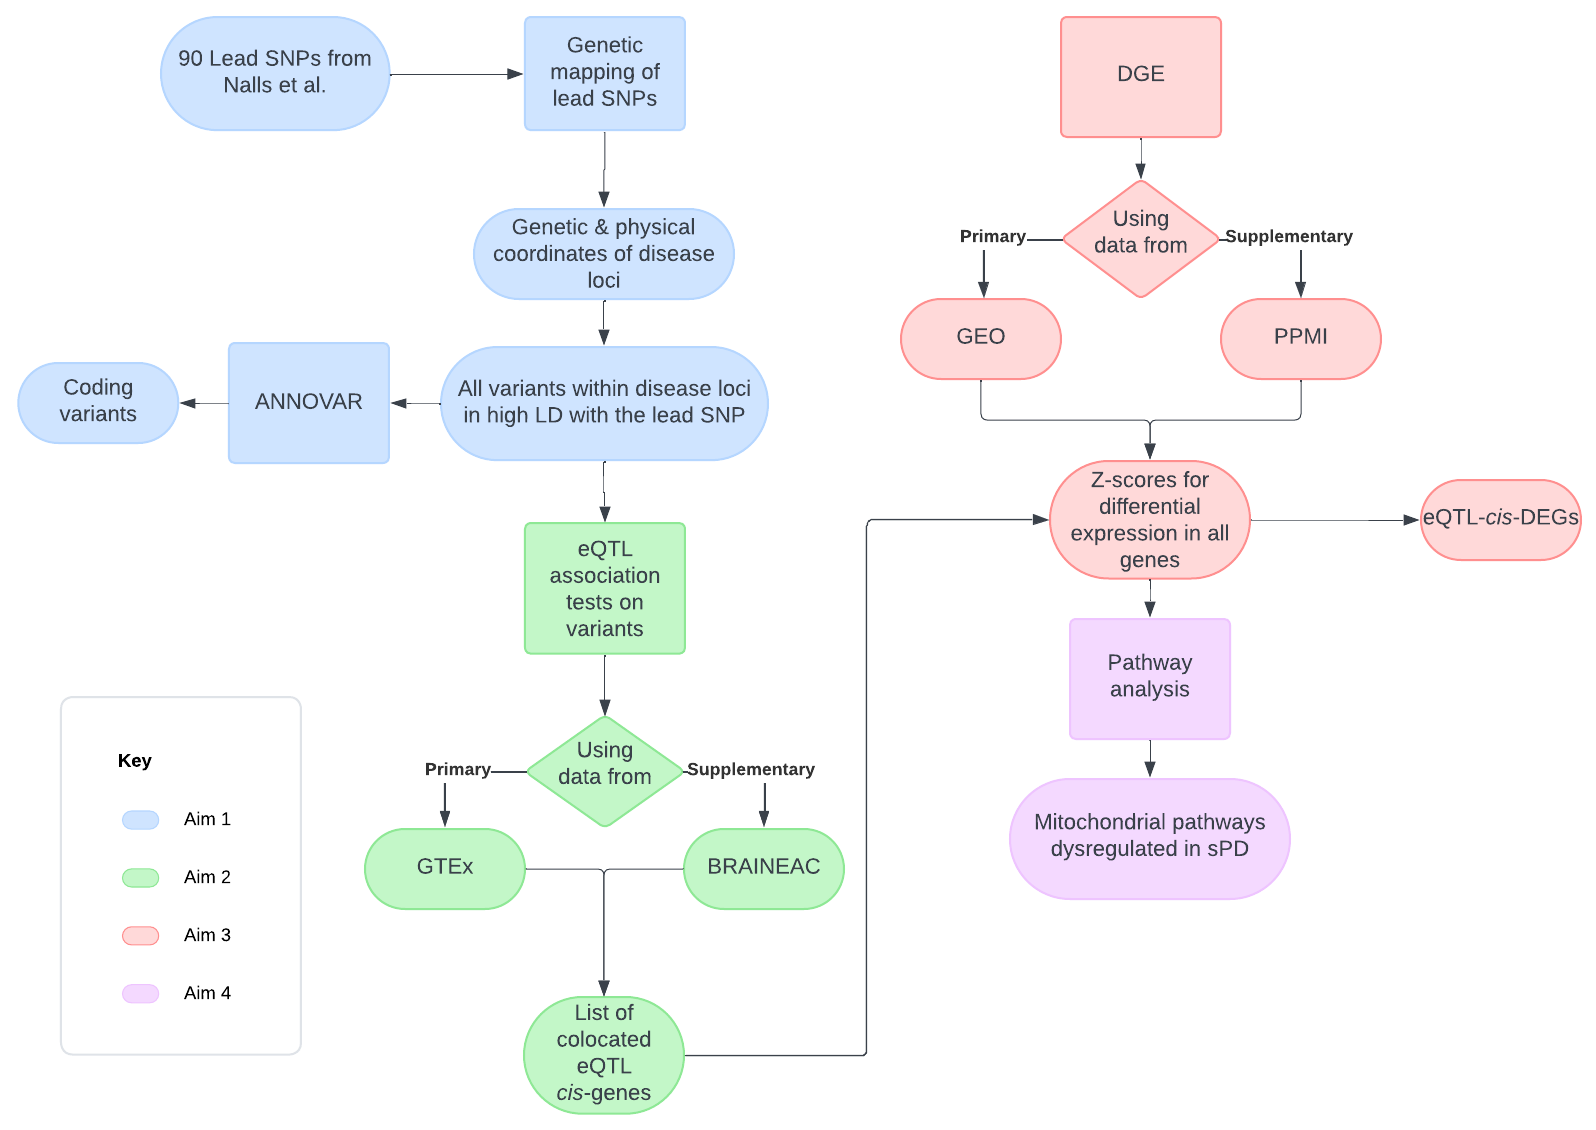
\includegraphics[width=1\linewidth]{Thesis/thesis images/MSc Flowchart.png}
    \caption{Project workflow, with steps taken to address Aim 1 (mapping) in blue, Aim 2 (Co-localisation) in green, Aim 3 (DGE analysis) in red, and Aim 4 (pathway analysis) in purple.}
    \label{fig:enter-label}
\end{figure}
%TC:endignore
In summary, this study aims to test the hypothesis that disease loci confer risk of sPD by the dysregulation of neighbouring \textit{cis}-genes. This is done by precisely co-locating eQTLs within stringently defined disease loci that are associated with \textit{cis}-genes $\pm$1.5Mb from the disease loci to find candidate target functional genes. Then, validate these genes and conduct pathway analysis of 43 mitochondrial pathways using DGE analysis data between sPD patients and healthy controls.
\newpage
\section{Materials and Methods}
\subsection{Characterisation of sPD disease loci}
\subsubsection{Identifying Lead SNP Information}
\label{subsubsec:SNPs}
The summary statistics for each of the 90 lead SNPs were collated from the Nalls et al. 2019 paper\cite{Nalls2019IdentificationStudies}. The physical coordinates of the lead SNPs were provided in the human genome build 37 format (GRCh37). In order to locate the genetic position of the lead SNPs, this project employed a high resolution genetic map\cite{Maniatis2004PositionalDisequilibrium.} based upon European HapMap 3 data. This map contains the genetic (in cumulative linkage disequilibrium units (LDU)) and physical coordinates (in kb) for 2110487 variants. All SNPs were therefore placed on cumulative LDU genetic coordinates, and physical coordinates on build 35 (NCBI35) of the human genome. To match the datasets together, the UCSC liftover tool\cite{Hinrichs2006The2006.} was used to convert the physical coordinates of the genetic map into build 37 format. 52861 variants were lost in the process, but since this only represents a small fraction of the overall dataset (2.5\%) this was deemed acceptable. The map now included the physical and genetic coordinates of 2057626 variants across the genome. Then, the Nalls et al.\cite{Nalls2019IdentificationStudies} lead SNPs were identified in this dataset. 30 of the lead SNPs were already located on the map and no further action was needed. The remaining 60 lead SNPs did not have genetic coordinates on this map, so the mean of genetic coordinates of the closest variant upstream and downstream were used as an estimated genetic coordinate for the lead SNP.
\subsubsection{Coordinates for Disease Loci Linkage Disequilibrium Blocks}
\label{subsubsec:LDblock}
The basis of this study is co-location - for which, accurate location estimates of disease loci are crucial, as discussed in \hyperref[subsubsec:co-location]{section 2.4.3}. To facilitate this, European-population genetic maps were used to define the coordinates of LD breakdown around each of the lead SNPs, as described by Lau et al.\cite{Lau2017High-ResolutionEuropeans}. This provides a region of interest at each of the disease loci in physical and genetic terms which can be used for the co-location analysis. For most lead SNPs, the corresponding LD block was defined as all variants at the exact same genetic location, ($\pm0LDU$ from each other). The genetic map was then filtered to only contain variants with $\pm0LDU$ from each of the lead SNPs. 2 pairs of 2 lead SNPs (rs823118 \& rs11557080, rs62053943 \& rs117615688) had the same genetic coordinates, and were considered to be part of the same locus, reducing the total number of PD disease loci from 90 to 88. 12 loci did not have any variants $\pm0LDU$ either side of the lead SNP, partly as their coordinates had to be estimated, so the definition of an LD block was extended to $\pm0.1LDU$. One of these loci that neighbours \textit{SNCA} was extended further, as it is of particular interest, and is discussed further in section \hyperref[subsec:SNCA]{4.7}. After filtering all variants to only be within the genetic coordinates of the LD block, the physical coordinates of the first and last variant within each of the 88 blocks were used to define the boundaries of the blocks. 
\subsection{Identification of eQTL Associated \textit{Cis}-Genes}
\label{subsec:eQTL}
To address the second project aim of identifying functional \textit{cis}genes (see section \hyperref[subsubsec:Aims]{2.5.2}),  two gene expression databases were used for identification and replication of \textit{cis}-genes: the Genotype Tissue Expression (GTEx) project\cite{Lonsdale2013TheProject} and the Brain Expression Almanac (BRAINEAC)\cite{Ramasamy2014GeneticBrain}. Both of these databases are population based, and are not designed around any particular disease. Importantly for this study, they contain expression data and genotype data for each sample - which allows for the calculation of eQTLs (described in section \hyperref[subsubsec:QTL]{2.4.2}). These eQTLs are sourced from healthy population-based data, so for the purposes of this project it is assumed that identified \textit{cis}genes are also likely to be relevant to disease. This assumption is discussed by Umans et al.\cite{Umans2021WhereEQTLs}. Additionally, the relevance of discovered \textit{cis}-genes will be assessed by the validation steps in \hyperref[subsec:validation]{section 3.3}. All eQTLs were calculated from expression data in the SN, as this is the primary region of neuronal death in PD. We assume that expression changes in the SN itself are therefore most likely to influence sPD risk.
\subsubsection{GTEx}
\label{subsec:GTEx}
Normalised expression matrices and vcf genotype data were obtained from GTEx version 8. As the latest GTEx v8 data are based on hg38, the coordinates from section \hyperref[subsubsec:LDblock]{3.1.2} were first converted from hg37 using the UCSC liftover tool\cite{Hinrichs2006The2006.}. All variants within the updated coordinates were extracted from the GTEx V8 genotype data (dbgap study accession phs000424.v9.p2, file accession phg001219.v1) using vcftools\cite{Danecek2011TheVCFtools} to create a vcf file that contained genotype for all variants within the LD blocks for all 838 samples in GTEx.
\\
\\After subsetting to European samples only (715 of the 838 samples), using the phenotype information file (file accession pht002742.v9.p2), LD statistics were calculated for the variants in relation to the lead SNP of their block. This was performed using an additive model, with biallelic variants coded 0, 1, 2. The Pearson correlation coefficient was calculated pairwise between the lead SNP of a locus and all other variants in that locus. The variants with $R^2\geq0.8$ were retained for further analysis. For the two blocks with two lead SNPs, the test was performed for all the variants against each of the lead SNPs independently, and of the two pairwise $R^2$ estimates generated for each variant, the higher value was retained for the cutoff. This list of variants was screened using ANNOVAR\cite{Wang2010ANNOVAR:Data} to categorise them and search for any protein-altering mutations. 
\\
\\A total of 114 samples were available for SN expression data. Of these 114 samples, 101 were of European descent, and  7 of those 101 had either Alzheimer's or dementia, so were removed from this analysis. The remaining 94 samples were used in the analysis. The genotype file was subsetted to only contain the information for these 94 samples. The expression and genotype files were then converted to a suitable format, and the MatrixEQTL R package\cite{Shabalin2012MatrixOperations.} was then used to estimate association between each of the variants in high LD with the lead SNPs and the expression data for genes within 1.5Mb of the disease loci. Previous unpublished work by the lab qualitatively showed that a 1.5Mb search space captured most associated \textit{cis}-genes, without overextending into regions with fewer results. A nominal significance of $p\leq0.05$ was used to identify disease-eQTL \textit{cis}genes, as the primary aim of this analysis is precise genetic co-location. If either the lead SNP or a marker SNP in high LD with the lead SNP showed nominally significant evidence of association with a \textit{cis}gene, the variant and the \textit{cis}gene were saved as a putative disease-eQTL \textit{cis}gene pair. Five covariates were included in the eQTL regression: age, sex, ischemic time of sample, RNA Integrity Number (RIN) and smoking status. Age and sex were included as Nalls et al.\cite{Nalls2019IdentificationStudies} used these as part of their original design. Smoking status was used as it is known to be inversely correlated with PD\cite{Ben-Shlomo2024TheDisease}. Ischemic time, also called Post Mortem Index (PMI), is the time period between the death of the donor and the procedure applied to it. PMI was included as a linear regression model fitted using \textit{limma}\cite{Ritchie2015LimmaStudies} showed a significant correlation between PMI and the expression values of the sample.
\subsubsection{BRAINEAC}
To replicate the eQTL results from GTEx, another database was used: BRAINEAC\cite{Ramasamy2014GeneticBrain}, the data portal of the UK Brain Expression Consortium. It is a database exclusively focused on the brain, and has samples from 10 different tissues. Genotype and expression data were available for 69  European SN samples. The expression data were obtained in fastq format, which was was first aligned using STAR\cite{Dobin2013STAR:Aligner} to the transcriptome and the genome, which were obtained from the UCSC hg38 fasta file and the refGene annotation file for it, located in the \href{https://hgdownload.soe.ucsc.edu/goldenPath/hg38/bigZips/}{UCSC bigZips website}. After alignment, PCA analysis was performed to test for significant covariates, of which RIN was found to be significantly associated with PC2. Four total covariates were included to be consistent with the previous GTEx eQTL procedure: Age, Sex, PMI, and RIN. Smoking status was omitted as it was not available in the phenotype information file. RSEM\cite{Li2011RSEM:Genome} was used to calculate Transcripts Per Million for the samples. Expression data was processed and normalised using the protocol described by GTEx v8 supplementary materials\cite{Aguet2020TheTissues}, using edgeR\cite{Robinson2010ttedgeR/ttData} and an inverse normal transformation. Then, the formatted genotype and expression data was used to test for association in the same was as described in the \hyperref[subsec:GTEx]{previous section}.The most statistically significant marker SNP-\textit{cis}gene pair for each \textit{cis}gene at the disease loci defined by the LD blocks were identified. The two lists of unique significant eQTL \textit{cis}-genes from GTEx and BRAINEAC were compared for overlap, and combined for further analysis. 
\subsection{Differential Gene Expression (DGE) Analysis}
\label{subsec:validation}
The previous section describes the search for associations between the disease loci and \textit{cis}-genes in healthy population data. In order to then validate the identified eQTL \textit{cis}-genes for relevance to sPD, Differential Gene Expression (DGE) analysis  was performed. DGE analysis tests for difference in the mRNA expression levels of genes across at least 2 conditions, in this case healthy controls and disease patients. This analysis is conducted under the hypothesis that a change in transcript expression level is contributing the to onset or progression of sPD. By testing for DGE of disease locus co-located eQTL-\textit{cis}genes across controls and PD patients, DGE will highlight the \textit{cis}genes with potential to be responsible for phenotypic affects through differential expression. The analysis also serves as validation. Genes that show association with sPD in two independent ways (eQTL co-location and DGE) are more likely to be true positives involved in the disease than genes identified through a single method.  Two databases were used for DGE: the Gene Expression Omnibus (GEO), and FOUNDIN-PD. Both databases contain expression data and sPD status. This allows each gene to be tested for a significant difference in expression between the case and the control samples. Additionally, pathway analyses (described in section \hyperref[subsubsec:pathwaysandnetworks]{2.4.4}) require a ranking metric for computation of enrichment scores. The calculated Z-scores from DGE analysis will be used as the ranking metric for this study (see section \hyperref[subsec:pathways]{3.4} for more detail). 
\subsubsection{The GEO}
The GEO \cite{Barrett2012NCBISetsupdate} is a public repository for genomics data. This provides a platform for large-scale analysis of observational data for many diseases. As part of previous work by the group, a meta-analysis of 13 PD case-control expression datasets following the methodology described by Choi et al.\cite{Choi2003CombiningVariation}. The datasets were selected based on the brain region, the availability of the data and corresponding metadata (including PMI, RIN, age and sex), and the case-control study design. Of these thirteen, six of them were selected for further analysis, based on a correlation coefficient of $\geq0.3$ for genomic expression across four or more datasets. The studies were all specifically sPD, not fPD. Information about the samples are summarised in table 2.
%TC:ignore
\begin{table}[h]
    \hskip0cm
    \centering
    \caption{Summary information for the 6 studies used for meta-analysis including the GEO accession code, the tissue analysed, sequencing platform used, numbers of cases and controls, and availability of 4 covariates. All sequencing platforms are from Illumina.}
    \begin{tabular}{ |c|c|c|c|c|c|c|c|c|c| }
        \hline
        Accession & Tissue & Platform & Controls & Cases & Age & Sex & PMI & RIN \\ \hline
        GSE106608 & Subthalamic nucleus & HiSeq 2500 & 9 & 7 & Y & Y & N & N \\ \hline
        GSE133101 & Amygdala & NextSeq 500 & 26 & 43 & N & N & N & N \\ \hline
        GSE136666SN & Substantia nigra & HiSeq 2000 & 5 & 5 & N & Y & N & N \\ \hline
        GSE205450CAU & Caudate & NovaSeq 6000 & 40 & 35 & Y & Y & Y & Y \\ \hline
        GSE205450PUT & Putamen & NovaSeq 6000 & 41 & 34 & Y & Y & Y & Y \\ \hline
        GSE68719 & Prefrontal cortex & HiSeq 2000 & 44 & 29 & Y & Y & Y & Y \\ \hline
    \end{tabular}
    \label{tab:my_label}
\end{table}
%TC:endignore
\\From these six studies, meta-p values (nominal and adjusted) and meta-Z scores were calculated for differential expression between cases and controls using GeneMeta\cite{LusaL2024GeneMeta:Experiments.} and following similar methodology to that described in Maude et al. 2021\cite{Maude2021NewDiabetes.}.
\subsubsection{The PPMI}
The Parkinson's Progression Markers Initiative (PPMI)\cite{Marek2011ThePPMI} is a large-scale multinational consortium with multiple sub-studies. The data used in this study was accessed from a PPMI sub-study called FOUNDIN-PD\cite{Bressan2023TheMechanism}. This is a repository for induced Pluripotent Stem Cell (iPSC) data, differentiated from blood samples of PD patients and from healthy controls. The samples used were restricted to just those differentiated into dopaminergic neurons, to model the SN that is the main focus of this study. Data from the final time point, day 65, were used as for this project. Additionally, carriers of \textit{LRRK2}, \textit{GBA1} or \textit{SNCA} mutations were removed. 37 single cell RNA (scRNA) samples were selected, from which pseudobulk counts were generated for each cell type. Once the processing of the scRNA data were complete, DGE was performed on the cases against the controls using \textit{limma}\cite{Ritchie2015LimmaStudies}. This provided the p-values and Z-scores for each gene, which were used in section 3.3.3 and \hyperref[subsec:pathways]{3.4} respectively.
\subsubsection{Validation of Co-located \textit{Cis}-Genes}
In order to validate the results from section \hyperref[subsec:eQTL]{3.1}, the list of \textit{cis}-genes with a co-located eQTL was cross-referenced to the DGE results from both GEO and PPMI. The list of final candidate target genes was constructed of \textit{cis}-genes that had both a co-located eQTL from either GTEx or BRAINEAC, and showed significant ($p\leq0.05$) evidence of differential expression between sPD cases and controls in either the GEO or PPMI results. These \textit{cis}-genes which are both Differentially  Expressed Genes (DEGs) and have a co-located eQTL are referred to as ``eQTL-\textit{cis}-DEGs" from here. This final list of eQTL-\textit{cis}-DEGs was also cross referenced with the IMPI dataset\cite{Smith2016MitoMinerDatabase} to determine which genes were localised to, associated with, or ancillary to, the mitochondrion.
\subsection{Pathway \& Network Analyses}
\label{subsec:pathways}
As described in section \hyperref[subsubsec:pathwaysandnetworks]{2.4.4}, pathway analyses are used to test for enrichment within pre-defined gene sets. The specific pathway analysis used here, GSEA, tested for either up or down regulation of the pre-defined gene sets. This is performed by computing a ranking metric, and testing for enrichment of the gene set at either the top or bottom of the ranking. In this study, GSEA was performed using the fgsea\cite{KorotkevichG2019FastAnalysis} R package. The gene sets tested were 43 clearly defined mitochondrial pathways, downloaded from MsigDB\cite{Liberzon2011Molecular3.0}, chosen based on their members having a high level of overlap ($\geq25\%$) with Mitocarta\cite{Rath2021MitoCarta3.0:Annotations}. These pathways represent many facets of mitochondrial function, including respiration, amino acid metabolism, and fatty acid metabolism. The ranking metric was defined as the complete list of Z-scores dervied from the DGE (section \hyperref[subsec:validation]{3.3}). Therefore, two independent GSEAs were performed - one using the Z-scores from the GEO DGE results, and one using the PPMI DGE results. The same gene sets were used for both. As the ranking metric was based on Z-scores, this meant that genes that are highly differential expressed between cases and control will be positioned at either end of the ranking. Genes that are upregulated in cases will be at the top of the list, and downregulated genes will be at the bottom. 
\\
\\Along with the GSEA pathway analysis, a network analysis was also performed using STRING\cite{Szklarczyk2023TheInterest}. This tool searches for known and predicted interactions between the members of a supplied list of proteins. Both functional and physical interactions were searched for, using all sources. The minimum confidence level of the interaction was the medium value of 0.4. The supplied list of proteins was derived from the 151 eQTL-\textit{cis}-DEGs from section \hyperref[subsec:validation]{3.3.3}. 10 of these genes did not have a corresponding protein, as they are ncRNA genes. Therefore, the total number of proteins within the network analysis was 141.
\newpage
\section{Results}
\subsection{Physical Coordinates of sPD Disease Loci}
\label{subsec:blocks}
The first aim of this study was to characterise disease loci for PD, based on the 90 lead SNPs identified by Nalls et al.\cite{Nalls2019IdentificationStudies}. Within their study, Nalls et al. identified the lead SNPs for sPD and their physical location. Using this information, we defined the genetic location of the lead SNPS. Then, we identified the physical coordinates of the region of LD around each lead SNP. A total of 88 disease loci LD blocks were stringently defined, based on a European population genetic map (derived from HapMap3 CEPH data)\cite{Maniatis2004PositionalDisequilibrium.}.
\\
\\In the primary dataset, all variants neighbouring the lead SNPs on were on the same LD block - $\pm 0$ LDU from each other. An additional dataset based on $\pm 0.5$ LDU was generated to identify wider LD block and step information where necessary. The count of LD blocks was reduced from the original 90 lead SNPs, as 2 pairs of 2 lead SNPs were in close proximity, and within the same LD block. The complete information and location estimates for the blocks are available \href{https://github.com/Thomas-brightwell/PD-MSc-project-code/blob/main/Thesis/Supplementary%20materials/Supplementary%20Results%20table%20.csv}{here}. The distribution of LD block sizes are summarised in Table 3 and \hyperref[fig:blockscatter]{Figure 4}. Table 3 shows the summary of genetic length (measured in additive LD units), the physical length, and the number of variants per block.
%TC:ignore
\begin{table}[!h]
\centering
\caption{Summary information for defined sPD disease loci LD blocks, including the sizes and number of variants within.}
\label{tab:sPDblocks}
\begin{tabular}{|l|ll|ll|}
\hline
       & \multicolumn{2}{c|}{Width}                & \multicolumn{2}{c|}{Variants (n)}    \\ \hline
       & \multicolumn{1}{l|}{Kilobases} & LD units & \multicolumn{1}{l|}{Total} & High LD \\ \hline
Mean   & \multicolumn{1}{l|}{38.2}      & 0.03     & \multicolumn{1}{l|}{640.7} & 18.8    \\ \hline
Median & \multicolumn{1}{l|}{25.3}      & 0.00     & \multicolumn{1}{l|}{392}   & 5.5     \\ \hline
Min    & \multicolumn{1}{l|}{0.4}       & 0.00     & \multicolumn{1}{l|}{13}    & 1       \\ \hline
Max    & \multicolumn{1}{l|}{247.1}     & 0.92     & \multicolumn{1}{l|}{6026}  & 295     \\ \hline
\end{tabular}
\end{table}
%TC:endignore
\\The mean length in kb of the LD blocks was 38.2kb, which is a much smaller region than most studies define as a single locus. As an example, Nalls et al.\cite{Nalls2019IdentificationStudies} defined variants as within a single locus if they were $\pm 250kb$ from each other. This highlights the specificity that the genetic maps provide this study. However, the locations themselves are not sufficient to unambiguously identify causal variants, as they will contain multiple potential haplotypes. Variants not only need to be within the LD block, but also in the risk haplotype. We assume in this study that variants in high LD with the lead SNPs are on this risk haplotype (threshold of $R^2 \geq 0.8$). As shown in table 5, the total number of variants varies quite dramatically between the blocks (13 to 6026). The same is true for the number of variants in high LD with the lead SNP (1 to 295). The lead SN is always in high LD with itself, so blocks with 1 high LD variant only contain the lead SNP. This is an important factor to consider, as the total number of eQTL tests performed per locus influences the likelihood of obtaining positive results under the null hypothesis for the eQTL analysis. 
\\
\\To illustrate the distribution of block sizes, Figure 4 shows a scatterplot and histogram of the genetic (additive LD units) and physical (kb) lengths of the LD blocks.
%TC:ignore
\begin{figure}[!h]
    \centering
    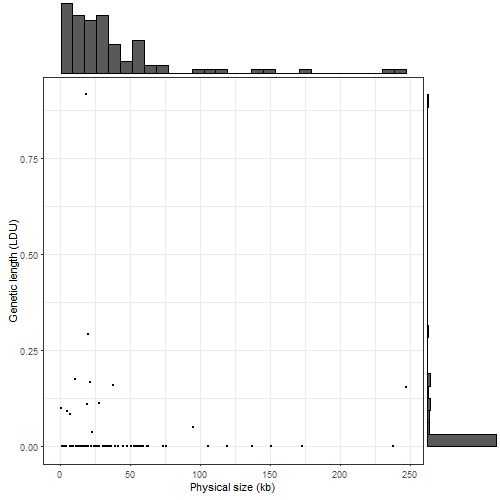
\includegraphics[width=1\linewidth]{Thesis/thesis images/blockscatter.png}
    \caption{Scatterplot with marginal histogram showing the frequency of different block sizes in genetic (LDU) and physical (kb) distance}
    \label{fig:blockscatter}
\end{figure}
%TC:endignore
\\The histogram highlights the two outliers that extend much farther than average size length of 38kb. These blocks represent stretches where there has been little historical recombination within the European population. It is potentially more challenging to identify functional variants within these large blocks, but this study focuses on the identification of neighbouring target (\pm1.5Mb) \textit{cis}-genes, which is described in section \hyperref[subsec:eQTLcoloc]{4.3}. 
\newpage
\subsection{Coding Variants}
\label{subsec:codingvariants}
Whilst it has been shown that GWAS variants which affect gene expression are most likely to be non-coding regulatory variants\cite{Nicolae2010Trait-AssociatedGWAS}, this is not the only mechanism by which variants can confer risk. To explore another route to risk, the LD blocks were screened for coding variants. These could act through differences in protein shape or function rather than gene expression level. One of the lead SNPs, rs34637584, was also identified in Nalls et al.\cite{Nalls2019IdentificationStudies} as a rare coding variant in the \textit{LRRK2} gene, and is reported in ClinVar as likely pathogenic for fPD. Whilst this variant may also be a plausible functional in sPD, the risk allele frequency in Europeans was too low for the population-based analyses in this study (<0.01). This meant calculating LD statistics was impossible, as there was no data for this variant in either the GTEx samples or the 1000 genomes project data. 
\\
\\Using ANNOVAR\cite{Wang2010ANNOVAR:Data}, a further 23 coding variants were identified that were in high LD with the lead SNPs and within the LD blocks, based on available 1000 genomes project data. 12 of these variants were synonymous, so were assumed to be benign (not presented). The remaining 11 missense variants may offer explanations for the associations detected at these loci. Pathogenicity of these variants was predicted and are presented in Table 4.
%TC:ignore
\begin{table}[h]
\centering
\caption{Missense variants in the disease loci, the gene and exon they are found within, the minor allele frequency, and pathogenicity predictions from 3 sources.}
\label{tab:codingvariants}
\begin{tabular}{|l|l|l|l|l|l|l|l|}
\hline
rsid        & LD block & Affected gene & Exon & MAF   & PolyPhen & SIFT     & CADD PHRED \\ \hline
rs76763715  & 3        & \textit{GBA1}           & 9    & 0.003 & 0.71     & 0.03     & 24.80 \\ \hline
rs34311866  & 22       & \textit{TMEM175}       & 9    & 0.286 & 0.00     & 0.03     & 8.91  \\ \hline
rs34813     & 33       & \textit{GIN1}          & 5    & 0.302 & 0.43     & 0.04     & 10.12 \\ \hline
rs757262    & 36       & \textit{TRIM40}        & 4    & 0.220 & 0.02     & 0.48     & 0.49  \\ \hline
rs757259    & 36       & \textit{TRIM40}        & 6    & 0.224 & 0.02     & 0.50     & 6.51  \\ \hline
rs112872773 & 37       & \textit{HLA-DRB5}      & 3    & 0.073 & 0.01     & 0.02     & 0.05  \\ \hline
rs2904880   & 70       & \textit{CD19}         & 3    & 0.314 & 0.00     & 0.14     & 7.70  \\ \hline
rs9938550   & 71       & \textit{HSD3B7}        & 7    & 0.362 & 0.00     & 0.62     & 4.03  \\ \hline
rs61742072  & 82       & \textit{DNAH17}        & 74   & 0.179 & 1.00     & No score & 2.83  \\ \hline
rs2282632   & 83       & \textit{ASXL3}         & 11   & 0.495 & 0.00     & 0.74     & 13.96 \\ \hline
rs41282950  & 87       & \textit{CRLS1}         & 4    & 0.126 & 0.95     & 0.65     & 27.40 \\ \hline
\end{tabular}
\end{table}
%TC:endignore
\\PolyPhen\cite{Adzhubei2010AMutations}, SIFT\cite{Ng2001PredictingSubstitutions}, and CADD\cite{Schubach2024CADDPredictions} are all tools to predict the effects of coding mutations on a protein. PolyPhen ranges from 0 to 1, with larger scores predicted as more deleterious. SIFT also ranges from 0 to 1, but in the inverse direction - closer to 0 is more deleterious. The CADD PHRED score is a scaled value, based on the ranking of all variants in the genome. The higher the score, the more deleterious the mutation is predicted to be.
\\
\\The full ANNOVAR table with information for all variants is available in the \href{https://github.com/Thomas-brightwell/PD-MSc-project-code/blob/main/Thesis/Supplementary%20materials/HighLDvariants.avinput.variant_function}{supplementary materials}, as well as the \href{https://github.com/Thomas-brightwell/PD-MSc-project-code/blob/main/Thesis/Supplementary%20materials/HighLDvariants.avinput.exonic_variant_function}{exonic variant table}, which only contains information for the exonic variants. Of the exonic missense variants, rs76763715 is the lead SNP for block 3. This block has no significant eQTL-\textit{cis}-genes. This variant is listed as pathogenic for both Gaucher disease and late-onset PD, and is in \textit{GBA1}, a major gene for PD (see section \hyperref[subsubsec:PDtypes]{2.1.2}). The pathogenicity predictions for some of these variants are not particularly strong, but it is important to note that under the common variant/common disease hypothesis, large effects are often not expected. A minor change in the protein may cumulatively influence disease susceptibility, along with many other factors.
\subsection{eQTL Co-location Analysis}
\label{subsec:eQTLcoloc}
The second aim of this study was to identify neighbouring (\pm1.5Mb) \textit{cis}-genes whose expression levels are influenced by the variants within the sPD loci defined in part \hyperref[subsec:blocks]{4.1}.The expression data used in this section from GTEx and BRAINEAC is population based. This means it primarily reflects healthy variation. However, by utilising the carefully defined disease loci, we can co-locate genes with eQTLs to these loci, making these \textit{cis}-genes are potentially relevant to sPD. This process allows us to identify candidate functional genes that can then be analysed further to directly associate with disease status through validation in section \hyperref[subsec:DGE]{4.4}. As outlined in section \hyperref[subsec:eQTL]{3.2}, eQTL associations with \textit{cis}-genes were tested using data from GTEx\cite{Aguet2020TheTissues} and BRAINEAC\cite{Ramasamy2014GeneticBrain}.
\\
\\For each sPD locus, all the variants in high LD with the lead SNP were tested for association with expression level of \textit{cis}-genes. The focus of this study is on the identified target genes, rather than the specific variants associated with them. Accordingly, unique \textit{cis}-genes with co-locating eQTLs were the primary result collated from the data. A total of 341 \textit{cis}-genes were identified as nominally significantly ($P \leq 0.05$) associated with at least one variant in high LD with the lead SNPs with the coordinates of the LD block. 73\% of the PD disease loci (64/88) we identified in section \hyperref[subsec:blocks]{4.1} had at least one significant co-located eQTL \textit{cis}-gene associated with one or more variants in high LD with the lead SNP for that locus (data available \href{https://github.com/Thomas-brightwell/PD-MSc-project-code/blob/main/Thesis/Supplementary%20materials/Supplementary%20Results%20table%20.csv}{here}). The numbers of unique eQTL \textit{cis}-genes per disease locus are summarised in table 5.
%TC:ignore
\begin{table}[h]
\centering
\caption{Summary information of co-location results, including the number of \textit{cis}-genes and variants per locus, and the relative eQTL abundance}
\label{tab:my-table}
\begin{tabular}{|l|ll|l|l|}
\hline
       & \multicolumn{2}{c|}{Cis genes (n)}       & Variants (n) & Relative (arb. unit) \\ \hline
       & \multicolumn{1}{l|}{Total} & Significant & high LD      & eQTL abundance       \\ \hline
Mean   & \multicolumn{1}{l|}{39.6}  & 3.9         & 18.8         & 12.6                 \\ \hline
Median & \multicolumn{1}{l|}{25}    & 2           & 5.5          & 4.1                  \\ \hline
Min    & \multicolumn{1}{l|}{4}     & 0           & 1            & 0                    \\ \hline
Max    & \multicolumn{1}{l|}{133}   & 31          & 295          & 78.9                 \\ \hline
\end{tabular}
\end{table}
%TC:endignore
\\From Table 5, similarly to the distribution of LD block sizes, the range of both cis-genes and high LD variants between blocks is quite large (127 \& 294, respectively). This will have an effect on the number of \textit{cis}-genes with a nominally significant co-located eQTL as more tests will inevitably produce more positive results. To indicate this, the relative eQTL abundance was also calculated as a function of block size:
\[ 
Relative\ eQTL\ abundance = \frac{eQTLs}{\textit{cis}-genes \times high\ LD\ variants \times 1000}
\]
\\This relative abundance showed the loci with the largest number of eQTL co-located \textit{cis}-genes proportional to the background of that loci were not the physically largest loci.
\label{fisher1}
Since the core hypothesis of this study relates to mitochondrial function, we classified all the identified eQTL-\textit{cis}-genes as NEMGs or not. A total of 23 eQTL-\textit{cis}-genes were NEMGs. To test for evidence of potential over-enrichment of NEMGs within the list of \textit{cis}-genes with a co-located eQTL, the total 2172 \textit{cis}-genes were divided into four groups, based on if they have a co-located eQTL (eQTL - or eQTL +), and if they are NEMGs or not (NEMG - or NEMG +). Counts for each group are displayed in table 6.
%TC:ignore
\begin{table}[h]
    \centering
    \caption{2X2 table used to calculate a Fisher's exact test, showing all \textit{cis}-genes, classified by NEMG and eQTL status.}
    \begin{tabular}{|l|l|l|l|}
        \hline
               & eQTL - & eQTL + & Sum  \\ \hline
        NEMG - &  1991    &  317    & 2308  \\ \hline
        NEMG + & 187   &  23  &  210\\ \hline
        Sum    & 2178   & 340    & 2518 \\ \hline
    \end{tabular}
\end{table}
%TC:endignore
\\A Fisher's exact test showed that there was no significant over-representation ($p = 0.29 \& OR = 0.77$) of mitochondrial genes in the eQTL-\textit{cis}-genes. The non-significant result is consistent with the null hypothesis. 
\subsection{Differential Gene Expression (DGE) Analysis}
\label{subsec:DGE}
The third aim of this study was to validate the candidate genes from the eQTL analysis, and directly link them to disease status. To this end, DGE analysis was conducted for two independent datasets - an observational meta-analysis of sPD studies from GEO\cite{Barrett2012NCBISetsupdate}, and an experimental iPSC sub-study of the PPMI called FOUNDIN-PD\cite{Bressan2023TheMechanism}. The validation process tested the \textit{cis}-genes with a co-located eQTL for differential expression between healthy controls and PD patients. These genes are eQTL-\textit{cis}-DEGs that have been validated to relate to both healthy variation and disease status. These represent the most probable target candidate genes for sPD risk. The overlap between the \textit{cis}-genes significant in the four databases (GTEx, BRAINEAC, GEO \& PPMI) used in this study is shown below in Figure 5.
\newpage
%TC:ignore
\begin{figure}[!h]
    \centering
    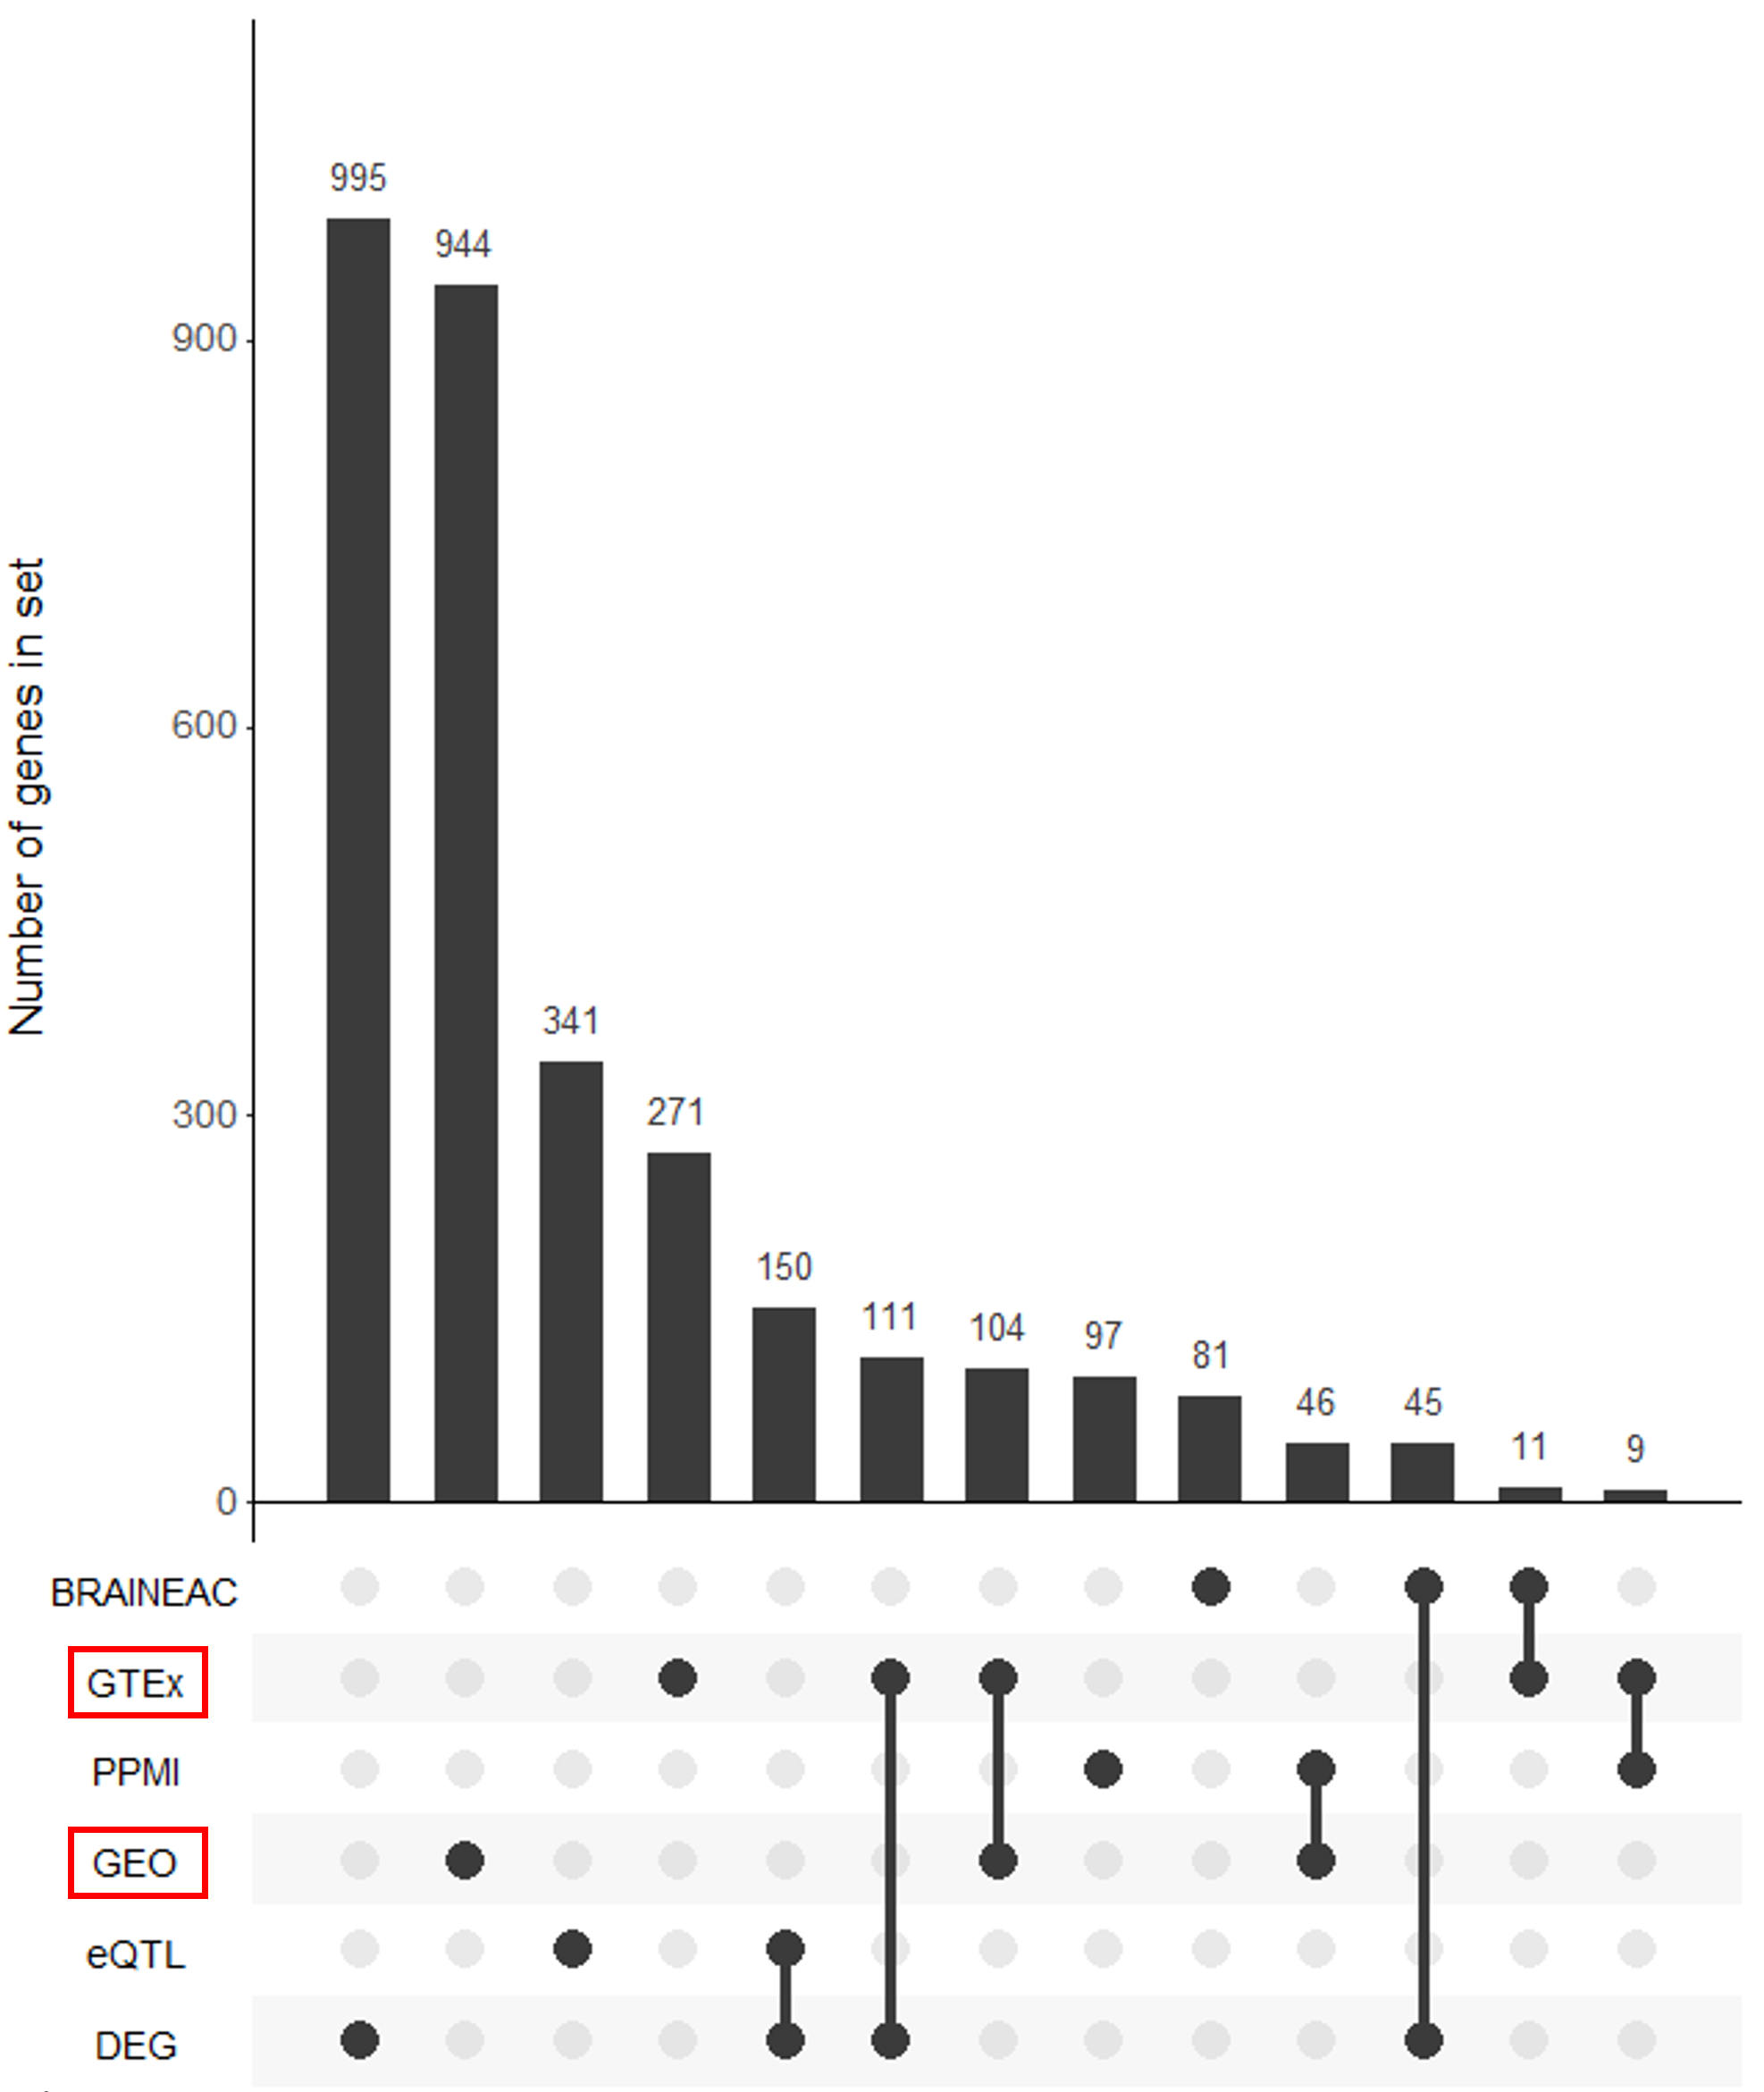
\includegraphics[width=1\linewidth]{Thesis/thesis images/Upsetplot.png}
    \caption{Upset plot\cite{Conway2017UpSetR:Properties.} showing overlap between nominally significant \textit{cis}-genes in the four databases (GTEx, BRAINEAC, GEO, and PPMI) and two combined categories of eQTL (eQTL found in GTEx or BRAINEAC) and DEG (significantly differentially expressed in GEO or PPMI). The primary datasets for eQTL analysis (GTEx) and validation of \textit{cis}-genes by differential expression by PD status (GEO) are highlighted}
    \label{fig:enter-label}
\end{figure}
%TC:endignore
\newpage
There were a total of 150 \textit{cis}-genes that showed both significant ($P \leq 0.05$) evidence of association with a variant in high LD with the lead SNP (the GTEx and BRAINEAC subsets), and significant ($P \leq 0.05$) evidence of differential expression between cases and controls (the GEO and PPMI subsets). Only 46 \textit{cis}-genes were significantly ($P \leq 0.05$) differentially expressed in both PPMI and GEO. There were no \textit{cis}-genes that were part of all 4 datasets. This disparity is explored further in the \hyperref[subsec:studydesign]{discussion}.
\\
\\To test if NEMGs were more likely to be DEGs than non-NEMGs within the subset of co-located eQTL \textit{cis}-genes, the total 341 \textit{cis}-genes with a co-located eQTL were divided into four groups, based on if they were NEMGs (NEMG - or NEMG +), and if they were DEGs (DEG - or DEG +). The totals for each group are shown in table 7.
%TC:ignore
\begin{table}[h]
    \centering
    \caption{2X2 table used to calculate a Fisher's exact test, showing all co-located eQTL \textit{cis}-genes, classified by NEMG and DEG status.}
    \begin{tabular}{|l|l|l|l|}
        \hline
                        & DEG - & DEG + & Sum \\ \hline
        NEMG - &  184   & 134   & 318  \\ \hline
        NEMG + &  7  & 16   & 23 \\ \hline
        Sum             & 191   & 150   & 341 \\ \hline
    \end{tabular}
\end{table}
%TC:endignore
\\A Fisher's exact test showed NEMGs were significantly over-represented as DEGs compared to non-DEGs ($p = 0.015\ \&\ OR = 3.13$). This contrasts with the previous result of no over-representation of mitochondrial genes in the eQTL results (see section \hyperref[fisher1]{4.3}). This potentially shows that whilst NEMGs are not more likely to have a co-located eQTL, of the NEMGs that do, they are more likely to be differentially express than non-NEMGs. This can be seen from the counts in table 7, since 42\% (134/318) of non-NEMGs are DEGs, but 70\% (16/23) of NEMGs are DEGs. The 16 mitochondrial eQTL-\textit{cis}-DEGs are shown below in Table 8, along with their potential role in sPD aetiology.
\begin{landscape}
\begin{table}[]
\centering
\caption{16 mitochondrial eQTL \textit{cis}-DEGs, their roles and potential relevance to PD, ranked by Z-score for differential expression by PD status from high to low. Z-scores were taken from the GEO meta-analysis for all genes aside from \textit{PKLR} \& \textit{UQCC2}, which were taken from the PPMI iPSC study.}
\label{tab:16genes}
\begin{tabular}{|p{1.5cm}|p{1cm}|p{1cm}|p{5cm}|p{5cm}|p{8cm}|}
\hline
Symbol   & Block & Z     & Name  & Function  & Relation to PD \\ \hline
\textit{BMP4}     & 65    & 6.50  & Bone Morphogenetic Protein 4       & Growth factor  & Involved in AD\cite{Wang2023BMP4HRMECs}. Aggravates mitochondrial dysfunction\cite{Zhang2021BMP4Disease} \\ \hline
\textit{SLC41A1}  & 6     & 4.72  & Solute Carrier Family 41 Member   1  & Sodium/magnesium transporter  & Previously associated with PD in   Chinese patients\cite{Wang2015GeneticPatients}\\ \hline
\textit{HAP1}     & 76    & 3.04  & Huntingtin Associated Protein  & Vesicular transport   & Involved in Huntington's and AD, may also be involved in PD\cite{Chen2023Huntingtin-associatedDiseases} \\ \hline
\textit{SLC25A39} & 77    & 2.86  & Solute Carrier Family 25 Member   39 & Imports glutathione across IMM  & Previously detected as a candidate gene for PD\cite{Gialluisi2021IdentificationDisease}. Glutathione is needed for oxidative phosphorylation\cite{Wang2021SLC25A39Cells}   \\ \hline
\textit{PKLR}     & 2     & 2.48  & Pyruvate Kinase L/R   & Pyruvate kinase  & Pyruvate metabolism is important   for PD\cite{Gray2014RegulationDisease}  \\ \hline
\textit{UQCC2}    & 37    & 2.48  & Ubiquinol-Cytochrome C Reductase   Complex Assembly Factor 2 & Required for assembly of complex   III & Complex III deficiency\cite{Tucker2013MutationsExpression}\\ \hline
\textit{SOCS3}    & 82    & 2.25  & Suppressor Of Cytokine Signaling   3   & Inhibits cytokine   signalling     & Regulates microglia\cite{Wang2024SOCS3Macrophages} \&   inflammation\cite{Woo2015ControlDiseases}\\ \hline
\textit{NDUFB6}   & 49    & -2.01 & NADH:Ubiquinone Oxidoreductase Subunit B6 & Subunit of complex I  & Complex I deficiency\cite{Loublier2011TheLines} \\ \hline
\textit{CDIPT}    & 70    & -2.14 & CDP-Diacylglycerol--Inositol   3-Phosphatidyltransferase     & Synthesis of PtdIns, which are   secondary messengers & PtdIns are involved in autophagy\cite{Zhang2021TargetingDisease} \\ \hline
\textit{CUTA}     & 37    & -2.38 & CutA Divalent Cation Tolerance   Homolog    & Anchors proteins to membranes  & Involved in APP and Aβ processing\cite{Hou2015TheGeneration}, which is potentially involved in PD\cite{Lim2019Amyloid-Disease} \\ \hline
\textit{TUBB}     & 36    & -2.39 & Tubulin Beta Class I  & Component of microtubules & Directly interacts with LRRK2\cite{Law2014AAcetylation}. Involved in vesicle trafficking\cite{Sferra2020TUBBDynamics}  \\ \hline
\textit{COA3}     & 76    & -3.09 & Cytochrome C Oxidase Assembly   Factor 3   & Regulates assembly of complex IV   & Complex IV is involved in apoptosis\cite{Vladimirov2013MolecularComplex} \& PD\cite{Li2021MitochondrialChain}. \\ \hline
\textit{SLC25A21} & 64    & -3.99 & Solute Carrier Family 25 Member   21  & Transports dicarobylates across   the IMM  & Involved in respiration, and   depletion leads to mitochondrial dysfunction and spinal muscular disease\cite{Boczonadi2018MitochondrialDisease} \\ \hline
\textit{GPAT2}    & 10    & -4.06 & Glycerol-3-Phosphate   Acyltransferase 2, Mitochondrial      & Lipid metabolism   & Involved in lipid metabolism relevant to PD - Cardiolipin\cite{Xicoy2019TheDisease.}, and lipid interactions with $\alpha-synuclein$\cite{Fanning2019LipidomicTreatment.}  \\ \hline
\textit{NDUFAF3}  & 16    & -4.82 & NADH:Ubiquinone Oxidoreductase   Complex Assembly Factor 3   & Required for assembly of complex   I   & Causes Leigh syndrome\cite{Baertling2017MutationsSyndrome}. This disorder shares heritability with PD\cite{Wahedi2023TranscriptomicGenes} \\ \hline
\textit{LAP3}     & 24    & -5.05 & Leucine Aminopeptidase 3  & Removes N-terminal hydrophobic AAs & Interactions with complex I subunit\cite{Guarani2014TIMMDC1/C3orf1Complex} \\ \hline
\end{tabular}
\end{table}
\end{landscape}
The roles these 16 genes play are diverse, but many of which have been implicated in  sPD. These include complex I. III \& IV components, mitochondrial transport proteins, inflammation regulators, and amino acid metabolism. All genes have a potential link to sPD, but the evidence for some is much more direct and concrete than others. The respiratory complex I components in are particularly relevant, due to the strong evidence of complex I in PD, as was discussed in section \hyperref[para:oxidative]{2.3.3}. Additionally, previous studies have identified \textit{SLC41A1} \& \textit{SLC25A39} as potential PD related genes. These 16 genes are discussed more in section \hyperref[subsec:wider]{5.4}.
\subsection{Pathway Analysis Results}
The fourth and final aim of this study is to use pathway analysis to test clearly pre-defined mitochondrial pathways for disruption in sPD patients. To achieve this, we used GSEA analysis on 43 mitochondrial gene sets from multiple sources, that represent major functional pathways in the mitochondria. This was conducted using the same two datasets as the DGE, so GSEA results were calculated using the Z-scores for all genes from GEO and PPMI from the section \hyperref[subsec:DGE]{4.4}. The full dataset of mitochondrial pathways tested is available \href{https://github.com/Thomas-brightwell/PD-MSc-project-code/blob/main/Thesis/Supplementary%20materials/mito43.gmt}{here}. 26 of these 43 mitochondrial pathways were significantly (FDR $\leq0.05$) down-regulated in the observational case-control expression data from the GEO, (full results available
\href{https://github.com/Thomas-brightwell/PD-MSc-project-code/blob/main/Thesis/Supplementary%20materials/GEO_gsea_results.csv}{here}), shown below in \hyperref[tab:pathways]{Table 9}.
%TC:ignore
\newpage
\begin{table}[h]
\centering
\label{tab:pathways}
\caption{Mitochondrial pathways significantly downregulated in PD patients, using the meta-analysed GEO data. Pathways are ranked by the Normalised Enrichment Score, NES, from high to low.}
\begin{tabular}{|l|l|l|l|l|}
\hline
Pathway source & Pathway name                                   & FDR      & NES   & Pathway size \\ \hline
Reactome       & Mitochondrial biogenesis                       & 2.68E-02 & -1.47 & 91           \\ \hline
KEGG           & Arginine \& Proline metabolism                 & 3.65E-02 & -1.51 & 51           \\ \hline
Reactome       & Fatty acid metabolism                          & 8.50E-03 & -1.53 & 161          \\ \hline
KEGG           & Tryptophan metabolsm                           & 4.12E-02 & -1.56 & 34           \\ \hline
Reactome       & Long chain fatty acyl-CoA synthesis            & 4.61E-02 & -1.59 & 22           \\ \hline
KEGG           & Propanoate metabolism                          & 1.96E-02 & -1.66 & 31           \\ \hline
KEGG           & Alanine, Aspartate \& Glutamate metabolism     & 1.30E-02 & -1.68 & 30           \\ \hline
Reactome       & Fatty acid beta-oxidation                      & 1.05E-02 & -1.71 & 36           \\ \hline
Reactome       & Biotin transport \& metabolism                 & 2.27E-02 & -1.74 & 11           \\ \hline
Reactome       & Ketone body metabolism                         & 1.30E-02 & -1.79 & 9            \\ \hline
Reactome       & Gluconeogenesis                                & 7.81E-03 & -1.81 & 31           \\ \hline
Reactome       & BCAA catabolism                                & 1.53E-02 & -1.85 & 21           \\ \hline
Reactome       & Mitochondrial TRNA aminoacylation              & 1.05E-02 & -1.89 & 21           \\ \hline
KEGG           & Pyruvate metabolism                            & 2.43E-03 & -1.9  & 38           \\ \hline
Reactome       & Metabolism of amino acids \& derivatives       & 7.44E-09 & -1.96 & 348          \\ \hline
Reactome       & Mitochondrial calcium ion transport            & 1.80E-03 & -1.97 & 23           \\ \hline
Reactome       & Mitochondrial protein import                   & 3.09E-04 & -2.01 & 65           \\ \hline
KEGG           & Butanoate metabolism                           & 4.78E-05 & -2.28 & 29           \\ \hline
KEGG           & BCAA catabolism                                & 2.97E-06 & -2.32 & 43           \\ \hline
KEGG           & Citric acid cycle                              & 1.54E-05 & -2.36 & 29           \\ \hline
Mootha         & Mitochondrial genes                            & 2.16E-22 & -2.46 & 435          \\ \hline
Wong           & Mitochondrial genes                            & 5.64E-20 & -2.73 & 216          \\ \hline
Reactome       & Respiratory electron transport                 & 6.31E-13 & -2.79 & 93           \\ \hline
Reactome       & Citric acid cycle and ETC                      & 4.20E-19 & -2.81 & 164          \\ \hline
KEGG           & Oxidative Phosphorylation                      & 1.12E-14 & -2.82 & 107          \\ \hline
Reactome       & Chemiosmotic ATP synthesis and heat generation & 7.58E-15 & -2.83 & 115          \\ \hline
\end{tabular}
\end{table}
%TC:endignore
These 26 pathways collectively represent a large number of mitochondrial functions. Most of these can be grouped into four overarching functions: amino acid metabolism, respiration, fatty acid metabolism, and mitochondrial maintenance. The four most downregulated pathways are all part of respiration - and particularly the ETC. There are some pathways that overlap - for example, both Reactome and KEGG have a Branch Chain Amino Acid catabolism pathway. Since they are concordant with each other, this reinforces the evidence that they are being downregulated. That 60\% of tested pathways are significantly downregulated shows the scale of mitochondrial dysfunction in the brains of sPD patients compared to controls. The causality of these results are discussed further in section
\hyperref[subsubsec:causality]{5.2}.
\\
\\By contrast, only 2 of the 43 mitochondrial pathways were significantly ($FDR \leq 0.05$) differentially expressed when tested using the iPSC expression data derived from PPMI (data available \href{https://github.com/Thomas-brightwell/PD-MSc-project-code/blob/main/Thesis/Supplementary%20materials/PPMI_gsea_results.csv}{here}). These two pathways, Reactome metabolism of amino acids and derivatives \& KEGG glycine, serine, and threonine metabolism, were both upregulated (NES = 2.17 \& 1.86 respectively). KEGG glycine, serine, and threonine metabolism was non-significantly upregulated in the GEO data (NES = 1.21 \& FDR = 0.23). However, the Reactome metabolism of amino acids pathway was significantly differentially expressed in both data sets, but in opposite directions (NES = -1.96 and 2.17 for GEO and PPMI respectively). This contradictory may be due to a lack of power in the PPMI dataset, explored further in section \hyperref[subsubsec:GEOandPPMI]{5.1.2}. As the GEO results were based on six studies with 150 controls, we deemed them more reliable than the PPMI iPSC data with only seven controls for SN data.
\subsection{Network Analysis Results}
As a supplementary analysis to the main aims, an exploratory network analysis was also conducted. This was performed using the eQTL-\textit{cis}-DEGs - \textit{cis}-genes that showed evidence of differential expression in sPD cases, and had a co-locating eQTL within the disease loci. As described in section \hyperref[subsubsec:pathwaysandnetworks]{2.4.4}, a network analysis lends itself more to discovery than hypothesis testing, which is why this was not included in the main aims of the study. However, the results are still potentially informative, and may reflect pathways and connections that we did not or cannot test for in the GSEA results. Using the 151 eQTL-\textit{cis}-DEGs identified in section \hyperref[subsec:DGE]{4.4}, the network analysis was performed using STRING\cite{Szklarczyk2023TheInterest}, and the results are shown in \hyperref[fig:network]{Figure 6}.
\\
\\This network analysis of the eQTL-\textit{cis}-DEGs showed there were significantly more interactions than would be expected for a random set of proteins from both the genome ($p = 3.76e-08$) and from all \textit{cis}-genes surrounding the 88 sPD disease loci ($p = 0.0007$). 
After k-means clustering was applied, the largest cluster gad 41 genes (shown in red in figure 6). This cluster significantly more interactions within the list of all 151 genes than expected ($p = 0.0008$).
This cluster was functionally enriched for 5 total GO Biological Processes. 3 of these were quite general - cellular component assembly, cellular component biogenesis, and protein-containing complex activity. The remaining two pathways were much more specific - establishment of protein localization to vacuole and protein transport to vacuole involved in ubiquitin-dependent protein catabolic process via the multivesicular body sorting pathway.
%TC:ignore
\newpage
\begin{landscape}
\begin{figure}[]
    \centering
    \includegraphics[width=1\linewidth]{Thesis/thesis images/network analysis.png}
    \caption{Network analysis showing connections between identified disease-eQTL-\textit{cis}-DEGs. Nodes represent proteins, and the lines between them represent interactions. Proteins are colour coded based on which cluster they are in.}
    \label{fig:network}
\end{figure}
\end{landscape}
\subsection{\textit{SNCA} as a potential eQTL-\textit{cis}-gene}
\label{subsec:SNCA}
As described in section \hyperref[subsubsec:synuclein]{2.3.2}, \textit{SNCA} is the gene that encodes for $\alpha$-synuclein, the protein that forms the main component of Lewy-Bodies. \textit{SNCA} is one of, if not the most, important genes for PD. It is therefore worth additional attention.
\\
\\Within the list of 151 eQTL-\textit{cis}-DEGs is the gene \textit{SNCA-AS1}, the anti-sense transcript for $\alpha$-synuclein. Due to the importance of $\alpha$-synuclein to PD, this prompted further investigation into why \textit{SNCA} itself was not also in the list. \textit{SNCA} is differentially expressed in the GEO dataset, and did have multiple significant eQTL associations. However, these associations were with variants within the shared LD block, but not in high LD with the lead SNP. When examining the genetic map for the LD blocks that were in proximity to \textit{SNCA}, blocks 28 and 29, it was found that there was a distinct step between the two blocks, as shown in Figure 7.
\begin{figure}[!h]
    \centering
    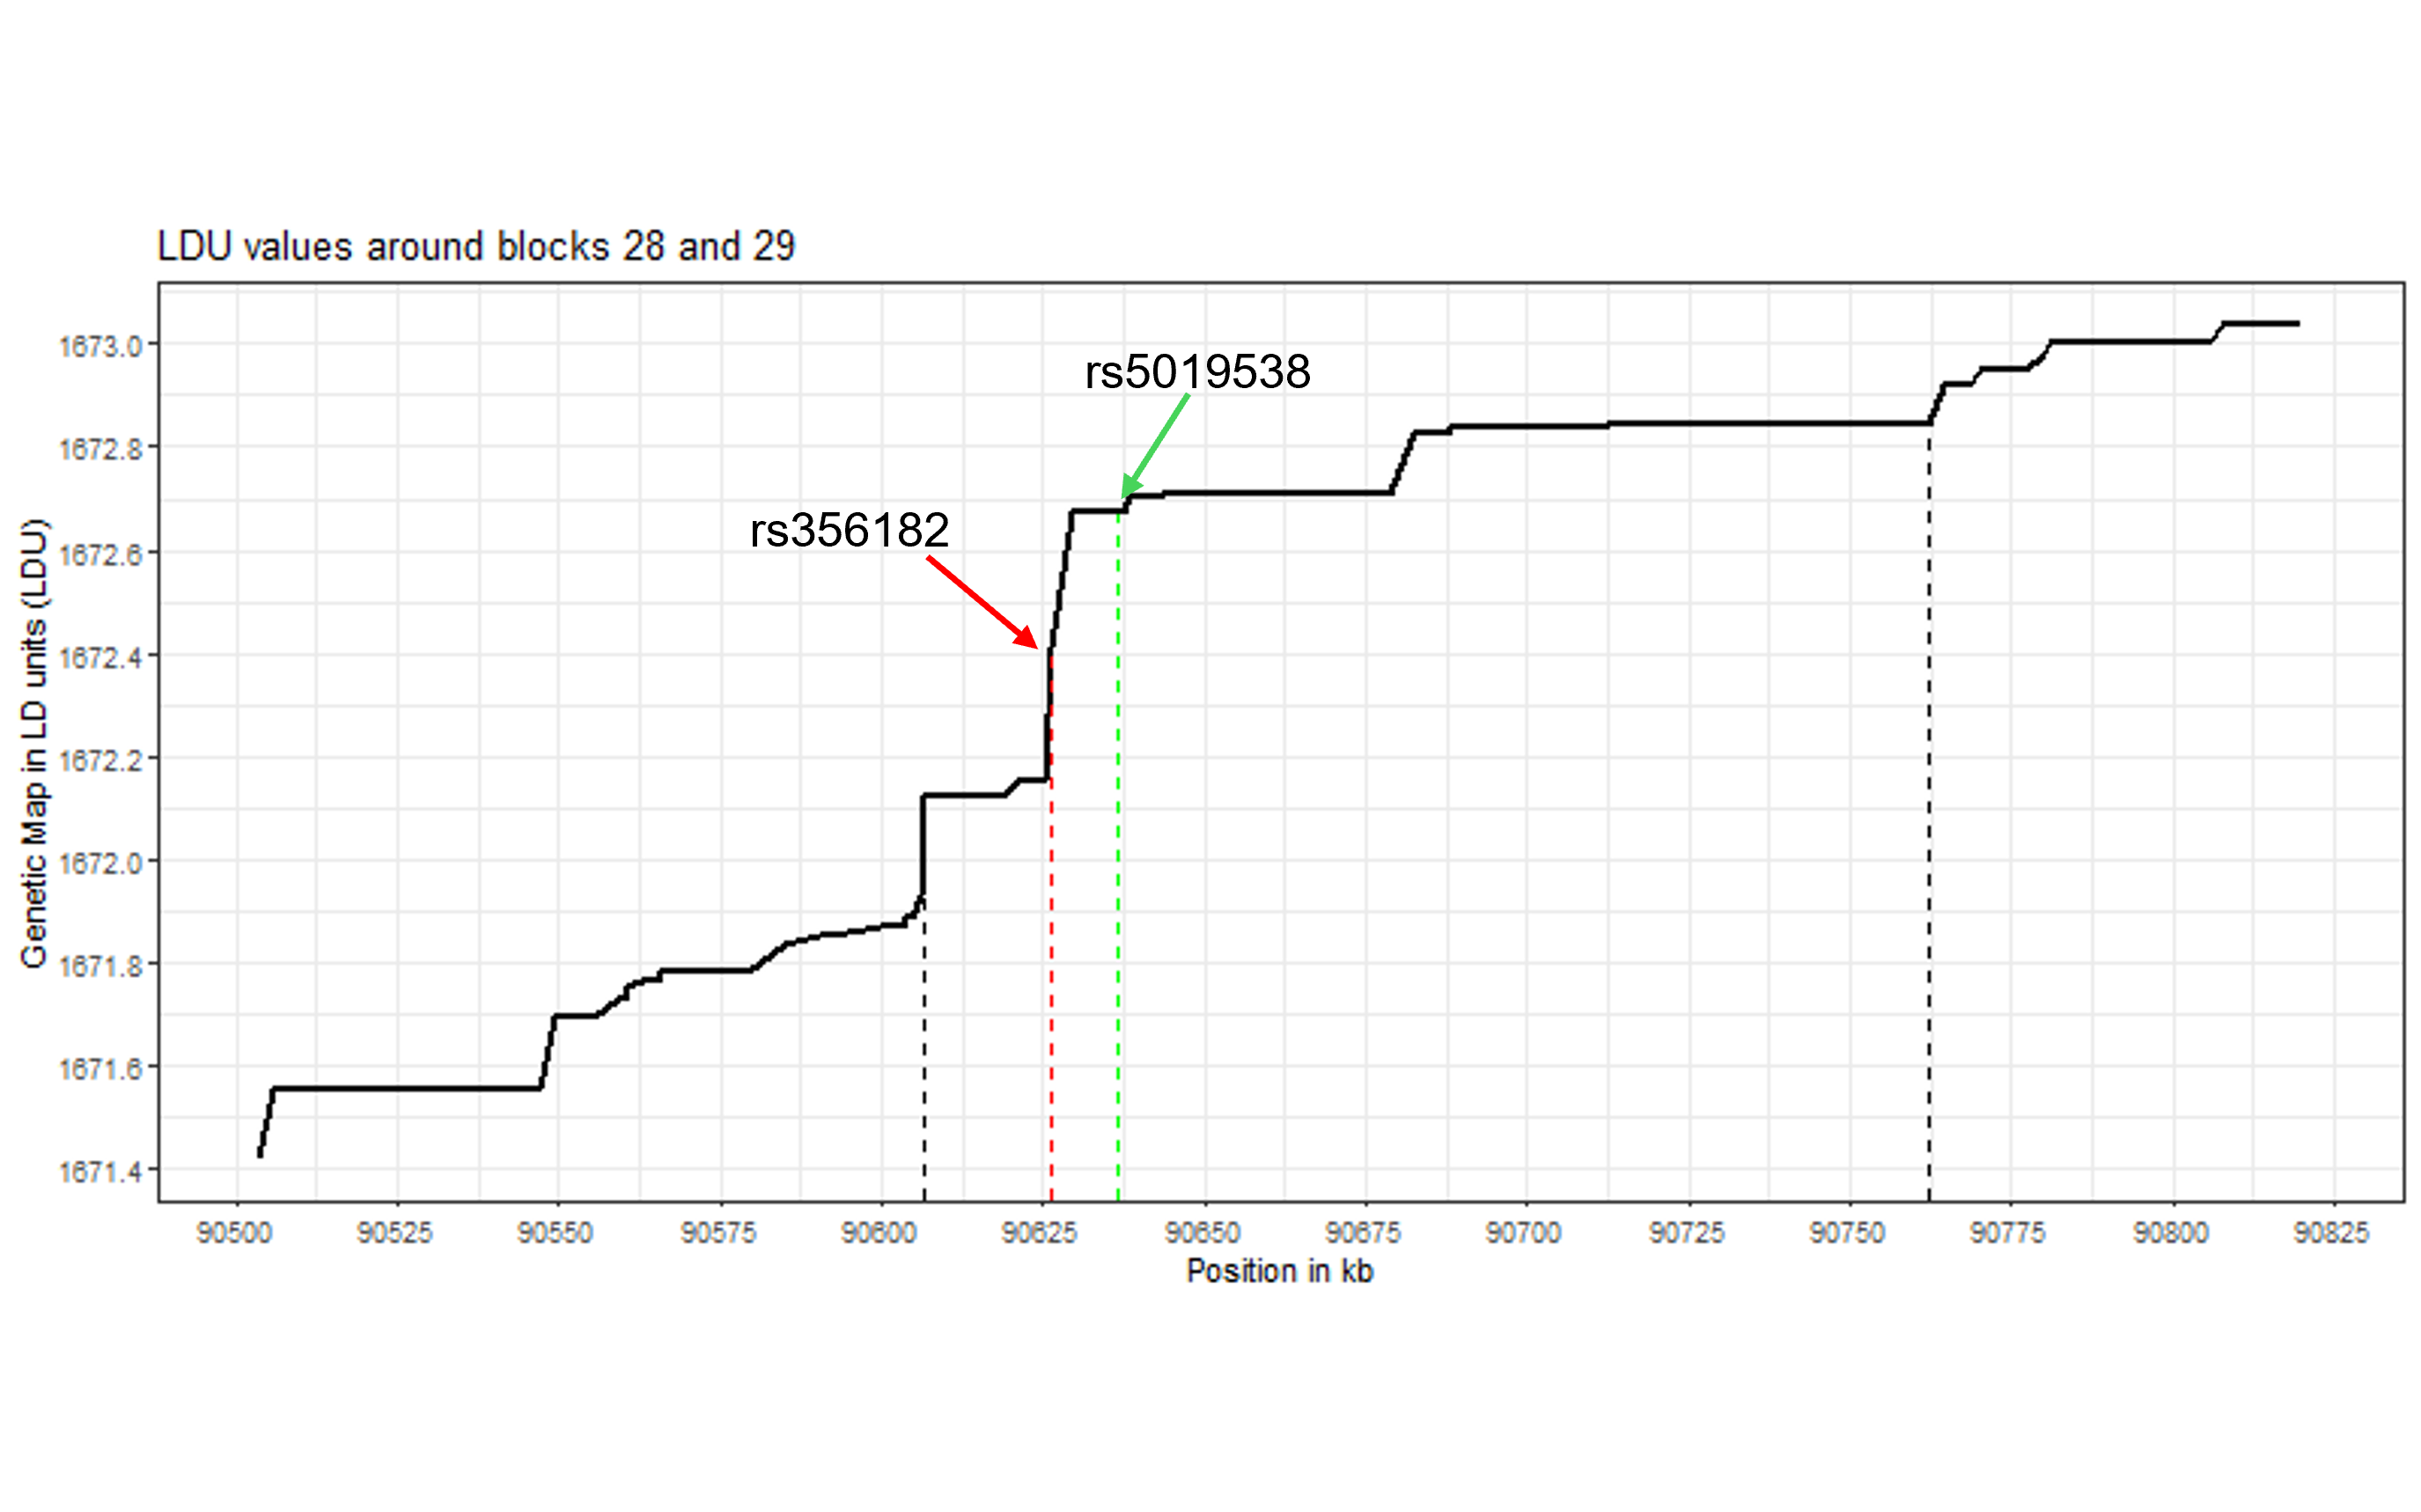
\includegraphics[width=1\linewidth]{Thesis/thesis images/Blocks28and29.png}
    \caption{Genetic map for blocks 28 and 29. The lead SNPs for blocks 28 and 29 (rs356182 \& rs5019538, respectively) are shown with the red and green dotted lines. rs356182 is located on a sharp vertical step. The boundaries of expanded combined region are shown by the black dotted lines.}
    \label{fig:blocks28and29}
\end{figure}
\\The genetic map unfortunately did not contain any variants in the 4kb step which where rs356182, lead SNP for block 28 is located. The genetic location of rs356182 had to be estimated as the midpoint of the two nearest variants on the map. This placed the lead SNP in an island with no variants in LDU0, and in the previous efforts, the variants that were 0.3 LDU  upstream were included in block 28. Upon re-examining this locus we decided to merge the two LD blocks and capture the region between the two dotted drawn lines drawn in Figure 7. This region had a total genetic length of 0.6 LDU, which is still a short genetic distance. The corresponding total physical length was 156 kb.
\\
\\The same process described in section \hyperref[subsubsec:SNPs]{3.1} was used identify the variants and calculate those in high LD with either lead SNP. It is worth noting that the 2 lead SNPs were in partial LD with each other, with an $R^2$ of 0.57. eQTLs for variants the extended region in high LD with the lead SNPs were processed (an additional 12 variants), and none of these showed association with \textit{SNCA}. There were some variants in linkage equilibrium with the lead SNPs ($largest R^2 = 0.0288$) that showed nominally significant evidence of association with \textit{SNCA} however. It therefore cannot be ruled out that variants in this are associated with \textit{SNCA}, but we have not found any markers in high LD with the lead SNPs that are associated with \textit{SNCA} expression.
\newpage
\section{Discussion}
\subsection{Study Design}
\label{subsec:studydesign}
\subsubsection{GTEx and BRAINEAC}
When considering the eQTL co-location results from both GTEx and BRAINEAC, we decided to take the combination of the results, not the intersection. This was largely due to the lack of overlap between the two datasets (just 11 genes, as shown in figure 5). Whilst it is possible that this is due to conflicting results, we believe that the GTEx co-location results are more robust when compared to the BRAINEAC data. Firstly, the BRAINEAC genotype data is derived from an older, array-based, sequencing method. The resulting coverage across the disease loci was accordingly much lower compared to GTEx's WGS approach, contrasting a total of 1620 high LD variants in GTEx to only 210 in BRAINEAC. This left some loci without any high LD variants in BRAINEAC, which may partially account for the limited overlap in eQTL-\textit{cis}-genes between the two databases. 
\\
\\The RIN scores for the BRAINEAC samples were also very low, with a mean score of 3.9. This is lower than the threshold GTEx used to discard expression data of 5.5\cite{Aguet2020TheTissues}. This means the BRAINEAC RNAseq is less reliable, as more RNA was degraded. This casts some doubt onto the integrity of results from the BRAINEAC dataset. These factors contributed to the decision to lead with GTEx as the main database for the eQTL analysis, with BRAINEAC only providing supplementary results. The potential risks of false positives from low-quality data are somewhat mitigated by the co-location study design, as a \textit{cis}-gene identified in BRAINEAC required evidence of differential expression and disease locus co-location to be included in the final list of candidate genes.
\subsubsection{GEO and PPMI}
\label{subsubsec:GEOandPPMI}
Whilst the GSEA results from the GEO database look quite promising, showing strong evidence of down-regulation of mitochondrial pathways in sPD patients, the replication failed for the PPMI dataset. Only 2 pathways showed significant dysregulation (and upregulated, not downregulated), and with far fewer genes significantly differentially expressed in PPMI compared to GEO (97 compared to 944). Whilst this reflects contradictory results, this is likely due to a lack of power for the PPMI data. There were only 7 control samples available for the PPMI data analyses. When combined with the differing study designs between two expression datasets used, it becomes hard to draw robust conclusions from comparisons between the two. Since using the iPSC data was an attempt to both replicate and validate the expression in one step, it may be better to separate these, and first replicate the downregulation of mitochondrial pathways observed in the GEO dataset using the same design, then separately validate it.
\subsection{Causality}
\label{subsubsec:causality}
A very difficult question to address is the causality involved in mitochondrial dysregulation. As discussed in section \hyperref[subsubsec:mitochondria]{2.3}, mitochondrial dysfunction is central to the development and progression of PD\cite{Bartman2024MitochondrialDiseases}\cite{MoradiVastegani2023MitochondrialStrategies}, but there is also evidence that mitochondrial dysfunction can be induced by $\alpha$-synuclein\cite{Sohrabi2023CommonDisease.}. This means mitochondrial dysfunction is likely both a cause and a consequence of PD. Considering this fact is important when analysing the GSEA results showing heavy mitochondrial pathway downregulation in the GEO dataset. The question is then, how do we know that these patients are suffering from sPD because they have this downregulation, and not that they have downregulation because they are suffering from sPD? 
\\
\\As part of our study design, we used GWAS lead SNPs from Nalls et al.\cite{Nalls2019IdentificationStudies} that relate to sPD status to define the disease loci. Then, in separate healthy variation databases (primarily GTEx\cite{Aguet2020TheTissues}), we searched for the effect of these loci on gene expression. In a perfect study, both of these analyses would be based upon data for the same samples. This would allow for direct combined eQTL analysis of disease loci in sPD patients specifically. It would also be beneficial for the analysis is PD cases were stratified more rigorously to reduce phenotypic heterogeneity. In particular, GBA1 mutation carriers should be identified, as they are often not distinguished from sPD\cite{Milenkovic2022GBADisease.}. This would remove a major confounding variable in the phenotypic profile of sPD patients. It may also be beneficial to harness longitudinal data if possible, as this could create gene expression profiles over the course of disease progression. This would clarify which genes are drivers and passengers in mitochondrial mutations, as the drivers should become misregulated earlier in the disease than the passengers. However, this would require data from either very early-stage sPD patients, or from population-based datasets with a large enough sample size to contain a usable number of sPD patients.
\subsection{Study context in the wider literature}
\label{subsec:wider}
Respiratory activity is a common thread between many of the results in this study. Of the 26 mitochondrial pathways downregulated (see Table 9), 6 of these were directly involved in respiration, from the ETC to glycolysis and the citric acid cycle. Additionally, of the 16 eQTL-\textit{cis}-DEGs (see table 8), 8 of them were involved in respiration. As discussed in section \hyperref[para:oxidative]{2.3.3}, respiration is clearly established to play a key role in PD, from complex I inhibitors\cite{Langston1983ChronicSynthesis} to ROS\cite{Subramaniam2013MitochondrialDisease}. One excellent candidate for further study from the eQTL-\textit{cis}-DEGs is therefore the complex I assembly factor \textit{NDUFAF3}. Rare mutations in this gene have been shown to cause complex I deficiency\cite{vanderVen2023ExpandingDisease} and neurological symptoms in affected patients. Complex I deficiency has been shown to result in increased oxidative stress\cite{Leman2015AssemblyDeficiency}, and as discussed in section \hyperref[para:oxidative]{2.3.2}, oxidative stress has strong evidence linking it to PD\cite{Subramaniam2013MitochondrialDisease}\cite{Gonzalez-Rodriguez2021DisruptionParkinsonism}.
\\
\\
Pyruvate metabolism is also implicated in both the eQTL-\textit{cis}-DEGs, and the downregulated pathways. \textit{PKLR} encodes for a protein kinase that is critical for glycolysis, and the KEGG pathway  Pyruvate is thought to be important for PD\cite{Gray2014RegulationDisease}, and it has been shown that pyruvate has a protective effect on models of PD\cite{Kim2022PyruvateDisease}. It is plausible then that a disruption of pyruvate metabolism may increase risk of sPD.
\\
\\As discussed in section \hyperref[subsec:inflammation]{2.2}, inflammation is a key factor in the propagation and progression sPD, specifically through microglia\cite{Isik2023MicrogliaDisease}. It is not surprising then that a gene like SOCS3 that regulates microglia\cite{Wang2024SOCS3Macrophages} is also a candidate functional gene. In a supplementary GSEA of KEGG pathways using the GEO data in WebGestalt\cite{Elizarraras2024WebGestaltMulti-omics} (download the report \href{https://github.com/Thomas-brightwell/PD-MSc-project-code/blob/main/Thesis/Supplementary%20materials/KEGG_GSEA.zip}{here}), it was also shown that inflammatory pathways were significantly upregulated in sPD patients. Inflammation ties back to the mitochondrion through apoptosis\cite{Vringer2023MitochondriaInflammation}, which is commonly achieved through mitochondrial membrane permeabilization.
\\
\\Cardiolipin is an important phospholipid in PD, which may also relate to some of the results. Cardiolipin is involved in $\alpha$-synuclein localisation to the mitochondria\cite{Ghio2016InteractionCardiolipin}, and in formation of mitochondrial pores in apoptosis\cite{Vringer2023MitochondriaInflammation}. This may explain how \textit{GPAT2} and the downregulated fatty acid metabolism pathways are linked to sPD. There is also evidence that associates fatty acid beta-oxidation to neuroinflammation and neurodegeneration\cite{Bogie2020FattyDisorders}, which could also explain the relevance of fatty acid metabolism to sPD.
\\
\\
The exploratory network analysis results show that the identified eQTL-\textit{cis}-DEGs are more interconnected than expected. The functional pathways enriched in the largest cluster are not particularly informative however, as cellular component assembly and biogenesis are broad terms. The biological processes that are enriched compared to the whole genome background are more interesting, indicating relation to the vacuole, but these may not be statistically valid conclusions. However, they are still interesting potential results, as vesicular trafficking was also highlighted in the eQTL-\textit{cis}-DEGs through \textit{HAP1} and \textit{TUBB}. Additionally, \textit{LRRK2} is also involved in vesicular trafficking\cite{Usmani2021TheDisease} and directly interacts with \textit{TUBB}\cite{Law2014AAcetylation}. It is possible then that these network analysis results are highlighting an enrichment of genes involved in processes related to autophagy (and by extension, mitophagy), which is known to play a role in PD\cite{Lizama2021NeuronalDisease}.
\subsection{Strengths and Limitations}
\paragraph{Common \& Rare Variation and Disease}
One difficultly faced by this study is the application of healthy variation to disease susceptibility. This study is largely predicated on disease risk being influenced by common variants at the disease loci. However, if the lead SNPs from Nalls et al.\cite{Nalls2019IdentificationStudies} are marking rare variants with large effects, it will reduce the power of some of our analyses. As 2 of the lead SNPs are rare coding variants (see section \hyperref[subsec:codingvariants]{4.2}), it seems quite likely that this may be the case for some loci. The true landscape of risk variants is likely a mix of both common variants with small effects, and rare variants with large effects. We have tried to address this for the publicly available variants with rsids (see section \hyperref[subsec:codingvariants]{4.2}), but a true rare variant analysis would require a specific study including stringently categorised sPD patient data and targeted sequencing. Nevertheless, this genetic mapping study is relevant for further rare variant investigations, as it refines the region that would require deep sequencing.
\paragraph{Functional Variants}By considering the entire disease locus as one entity, this becomes both a strength and a limitation of the study. We cannot fully answer questions about functional variants with this study design. However, we can identify putative functional \textit{cis}-genes for further analysis.  So long as the hypothesis holds true that the lead SNP is in high LD with the true functional variant(s), further analysis such as haplotype analysis could be combined with variant level analysis to improve accuracy\cite{Liang2020HaplotypePhenotypes}. 
\\
\\Additionally, we have mapped the disease loci very precisely, which make identifying the functional variant more feasible for many loci. Some loci had a length of less than 1kb, the smallest (block 84) being only 418bp long. A locus of this size would be a prime target for sequencing to determine the specific functional variant and would be very cost-effective compared to large-scale sequencing if the LD block had not been defined. Leaving the smallest LD blocks aside, the overall mean length of 38kb \& median of 25kb is much more precise than many follow-on studies from GWASs - e.g. the pipeline described by Mountjoy et al.\cite{Mountjoy2021AnLoci} considers a region of 500kb, and variants with an $R^2\geq0.5$ with the corresponding lead SNP. This allows for more specific and denser analysis to be conducted which improves results\cite{Giambartolomei2014BayesianStatistics}. By combining both co-location and DGE analysis, we created a list of eQTL-\textit{cis}-DEGs which we have the most confidence in as candidate target genes, as not only have they been co-located with an eQTL to the disease loci, they are also differentially expressed between PD cases and healthy controls
\subsection{Future Work}
The investigations in this study are based upon the premise that risk variants for sPD act through changes in gene expression levels. Whilst it has been shown that most functional variants from GWASs are non-coding and regulatory\cite{Maurano2012SystematicDNA}, there is more than one way a regulatory element can interact with a gene. For example, splicing regulatory elements may change what isoform of a protein is expressed, and can be investigated \textit{in silico}\cite{Tubeuf2020LargescaleElements}. Splicing variants could be integrated into this study's workflow by analysing splicing QTLs (sQTLs). A preliminary search using the publicly accessible data from the GTEx portal\cite{Aguet2020TheTissues} was conducted, and it showed no overlap between genes that had an eQTL and an sQTL. However, due to time constraints, the full data for sQTLs were not analysed fully, and so were not included in the results. Therefore, revisiting the sQTLs would be beneficial, and if the preliminary results remained true in the full data, may offer insights into some or all of the 28 loci that did not have any significant eQTL associations.
\\
\\The analysis in this study is based on European population data, but the methods described here could be applied to any population. Maude et al.\cite{Maude2021NewDiabetes.} analysed both European and African American data when applying similar methods used in this study to Type-2 diabetes. Accordingly, a supplementary analysis to this study would be to apply the methods to African populations. If this identified shared candidate target genes between populations, this would increase confidence in their association with sPD. 
\\
\\The most ideal solution to address some of the limitations of both the eQTL colocation and DGE analysis would be a bespoke dataset. This could include bulk and scRNAseq from the SN of real sPD patients and healthy controls, combined with whole genome sequencing and targeted sequencing of the disease loci. This would allow us to identify specific functional variants with the deep sequencing, and if the sample size was large enough, disease-specific eQTL associations could be tested for, which would help resolve the question of causality described in \hyperref[subsubsec:causality]{5.2}. This dataset would also be used to attempt replication of the pathway analysis results found in GEO using the RNAseq data. If scRNAseq was used then this could also identify dopaminergic neuron specific effects, as was attempted with the PPMI dataset here. 
\newpage
\section{Conclusion}
This study has:
\begin{enumerate}
    \item Characterised the regions of LD around 90 PD lead SNPs
    \item Conducted eQTL and DGE to identify eQTL-\textit{cis}-DEGs that are prime candidate genes
    \item Shown that of the eQTL-\textit{cis}-genes, the mitochondrially associated genes are more likely to be DEGs and that these mitochondrial eQTL-\textit{cis}-DEGs are relevant to sPD, based on the established literature of PD.
    \item Shown that there is downregulation of over half of the mitochondrial pathways tested in sPD patients
\end{enumerate}
This study provides strong evidence that for the disease loci with the mitochondrial eQTL-\textit{cis}-DEGs, sPD risk is conferred by misregulation of the mitochondrial genes associated with the disease loci, which leads to further mitochondrial downregulation and therefore the death of dopaminergic neurons and PD. However, while this is a plausible interpretation of the study results, it contingent on replication and validation through further study, including both prospective and functional.
\newpage
\section{Code Availability}
The full code used for all analyses in this study, the data files necessary for the analysis, and all supplementary results tables and figures are available in the GitHub repository for this project:
\\\href{https://github.com/Thomas-brightwell/PD-MSc-project-code/tree/main}{https://github.com/Thomas-brightwell/PD-MSc-project-code/tree/main}
\newpage
\begin{singlespace}
\printbibliography
\end{singlespace}
\end{document}